% Appendix A

\chapter{Additional plots for HF} % Main appendix title

\label{AppendixA} % For referencing this appendix elsewhere, use \ref{AppendixA}

\section{Chapter \ref{chap2HFsec}: \ratiosl in HF}

\begin{figure}[h!]
\centering
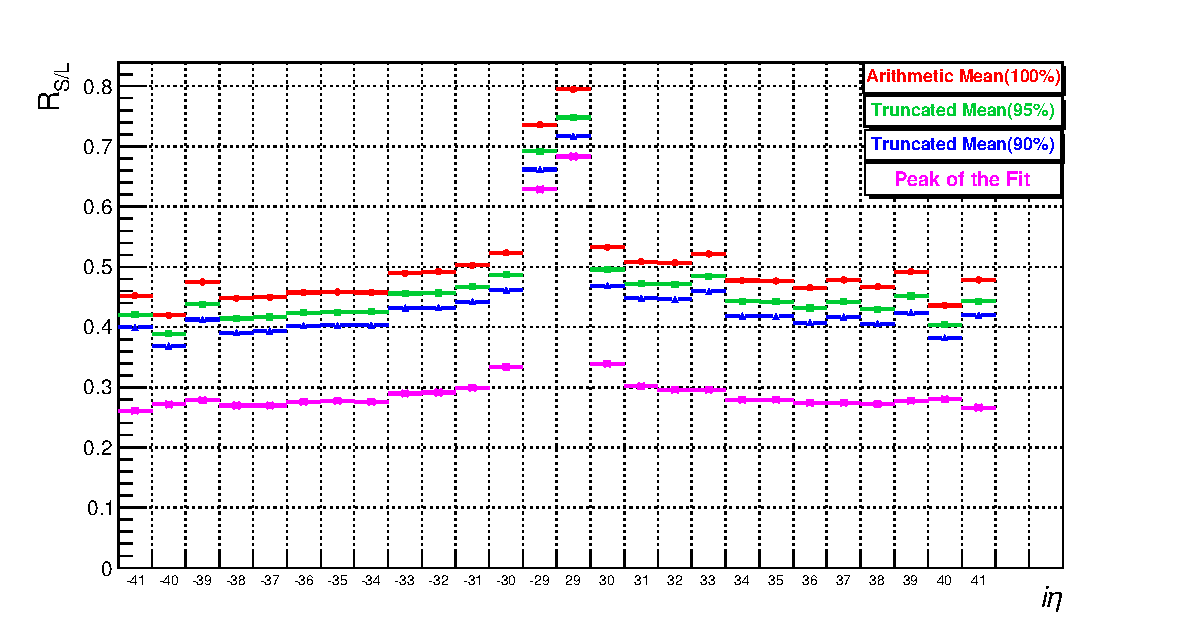
\includegraphics[width=0.8\linewidth]{../Figures/Chap2/ImageFiles_HF/Ratio/MeanvsFit.pdf}
\caption{\ratiosl vs $i \eta$}
\label{MeanvsFit}
\end{figure}


\begin{figure}[h]
\centering
%\includegraphics[width=0.99\linewidth]{../Figures/Chap2/ImageFiles_HF/Ratio/Ratioieta29to32.pdf}
%\includegraphics[width=0.99\linewidth]{../../../../../Figures/Chap2/ImageFiles_HF/Ratio/Ratioieta29to32.pdf}
\includegraphics[width=\linewidth]{../Figures/Chap2/ImageFiles_HF/Ratio/Ratioieta29to32.pdf}
%\includegraphics[width=0.99\linewidth]{figures/../Figures/Chap2/ImageFiles_HF/Ratio/Ratioieta29to32.pdf}
\caption{Asym. gaussian fit for \ratiosl ($|i\eta|$ 29 to 32)}
\label{fig:Ratioieta29to32}
\end{figure}
\begin{figure}[h]
\centering
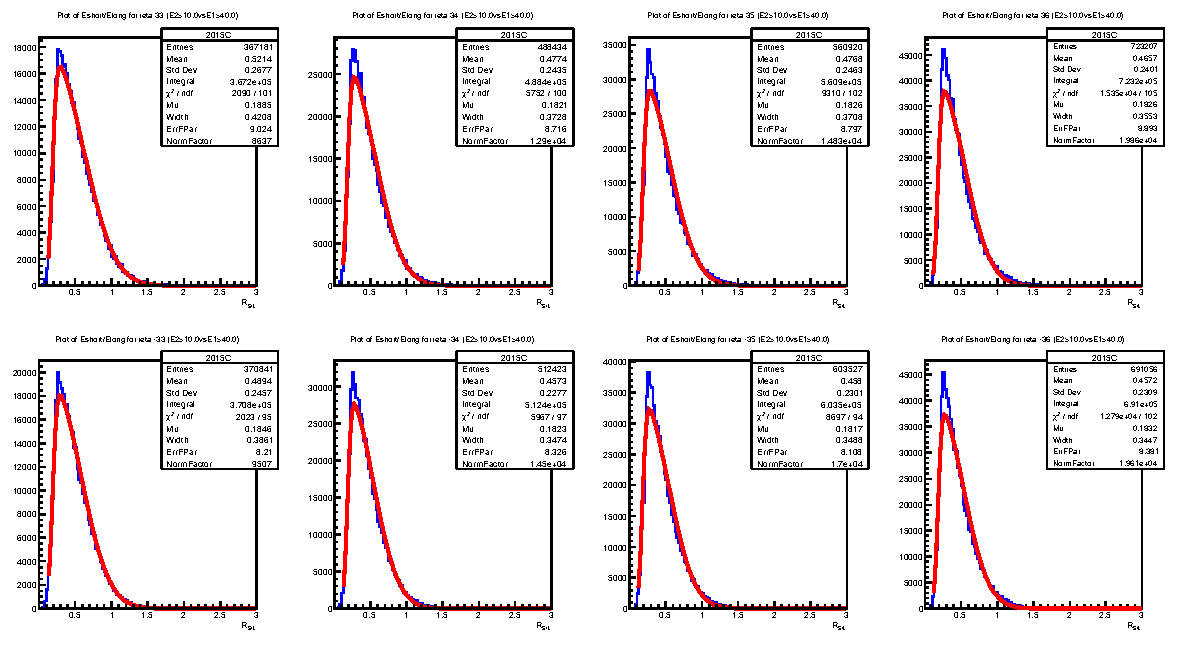
\includegraphics[width=\linewidth]{../Figures/Chap2/ImageFiles_HF/Ratio/Ratioieta33to36.pdf}
\caption{Asym. gaussian fit for \ratiosl ($|i\eta|$ 33 to 36)}
\label{fig:Ratioieta33to36}
\end{figure}
\begin{figure}[h]
\centering
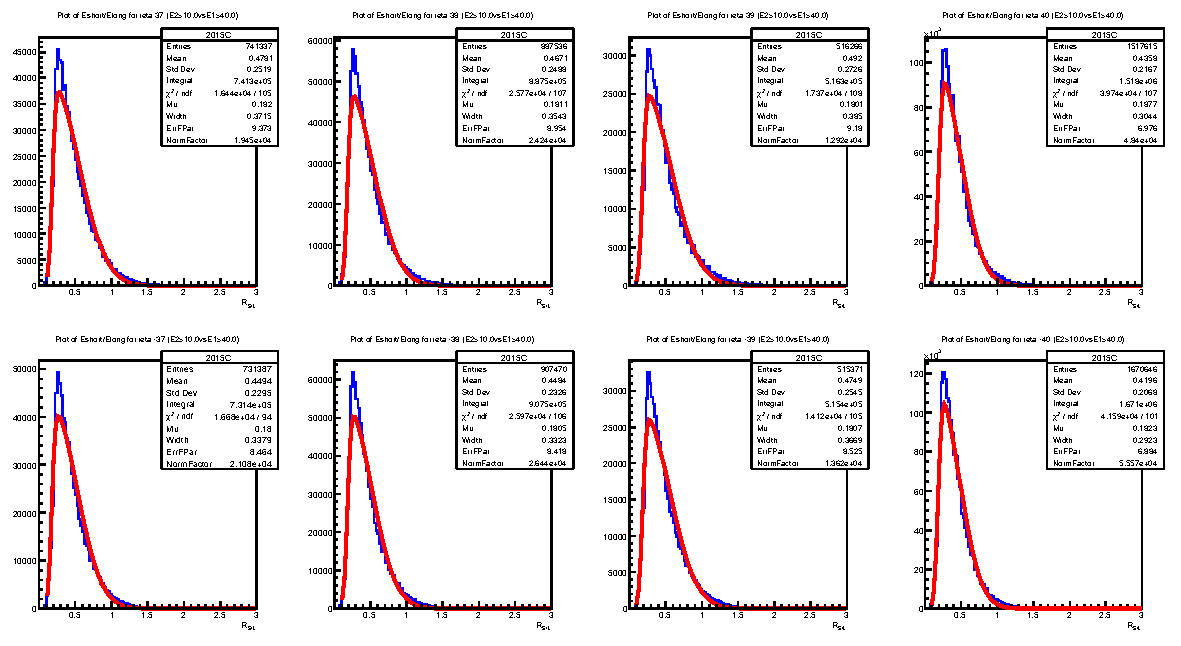
\includegraphics[width=\linewidth]{../Figures/Chap2/ImageFiles_HF/Ratio/Ratioieta37to40.pdf}
\caption{Asym. gaussian fit for \ratiosl ($|i\eta|$ 37 to 40)}
\label{fig:Ratioieta37to40}
\end{figure}
\begin{figure}[h]
\centering
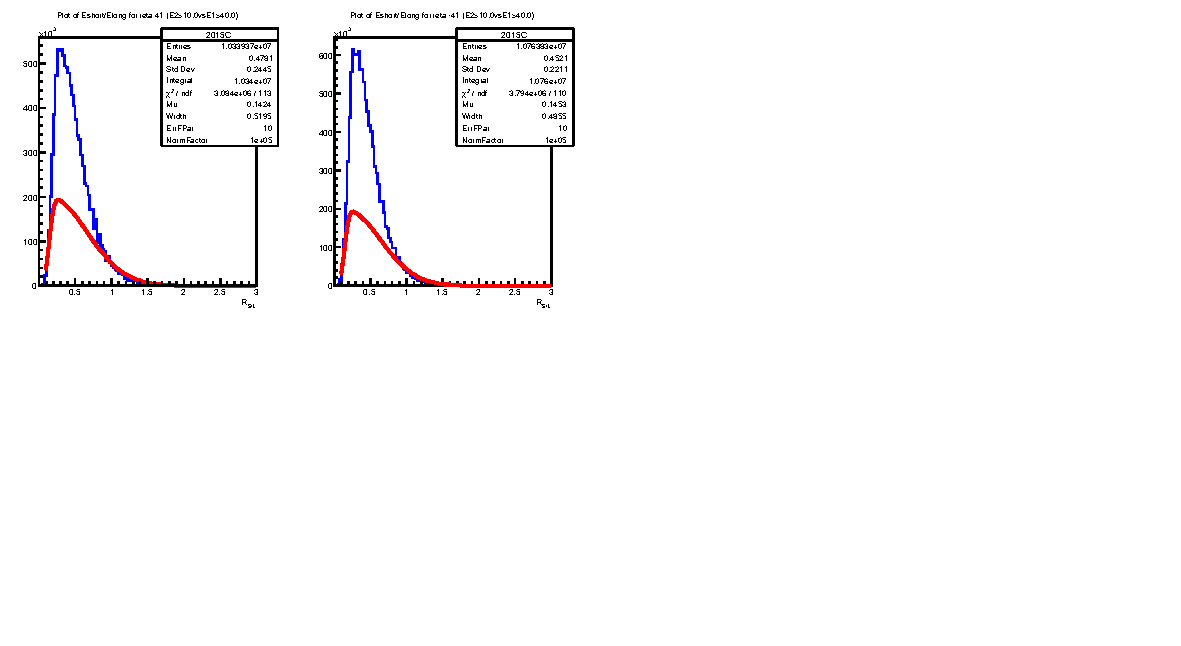
\includegraphics[width=\linewidth]{../Figures/Chap2/ImageFiles_HF/Ratio/Ratioieta41.pdf}
\caption{Asym. gaussian fit for \ratiosl ($|i\eta|$ 41)}
\label{fig:Ratioieta41}
\end{figure}


\begin{figure}[h!]
\centering
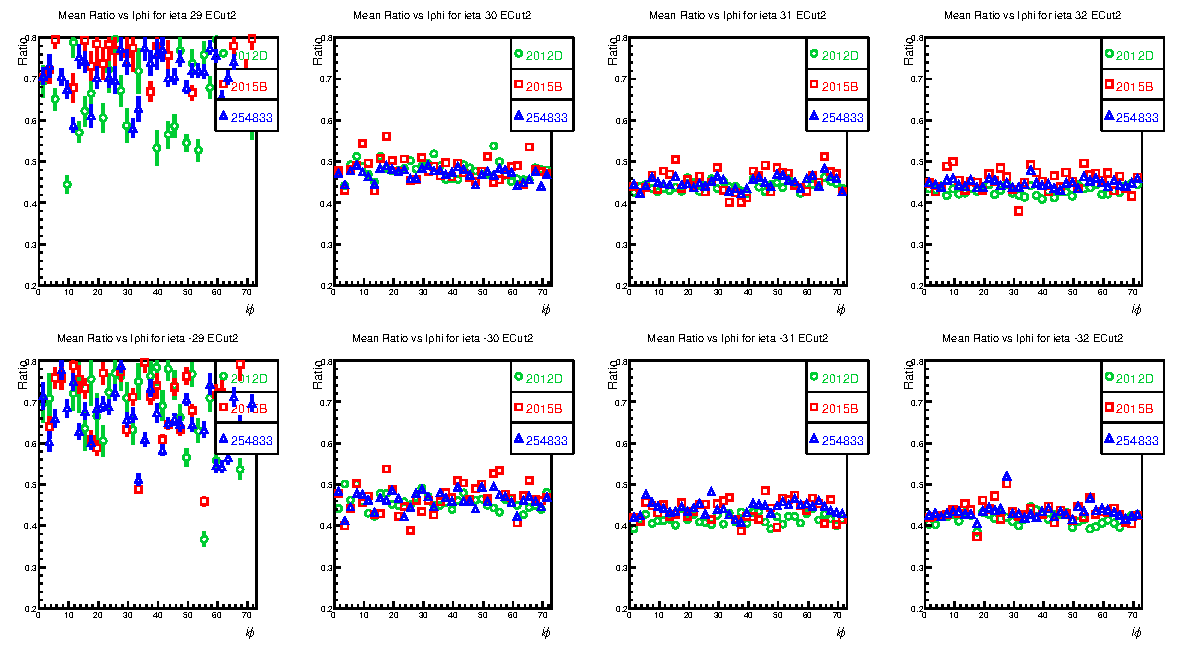
\includegraphics[width=0.99\linewidth]{../Figures/Chap2/ImageFiles_HF/2012vs2015/ieta29_32_E1E2Cut2Ietaiphi.pdf}
\caption{\ratiosl vs $i \phi$ for $|i\eta|$ 29 to 32}
\label{fig:ieta29_32_E1E2Cut2Ietaiphi}
\end{figure}
\begin{figure}[h!]
\centering
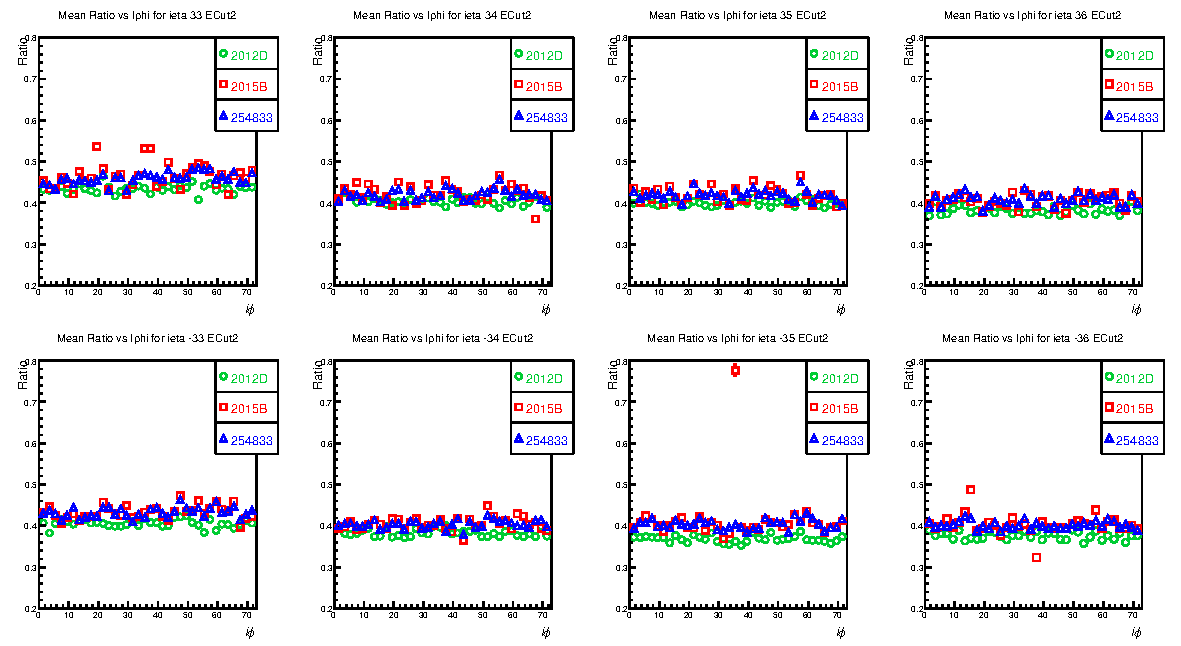
\includegraphics[width=0.99\linewidth]{../Figures/Chap2/ImageFiles_HF/2012vs2015/ieta33to36E1E2Cut2Ietaiphi.pdf}
\caption{\ratiosl vs $i \phi$ for $|i\eta|$ 33 to 36}
\label{fig:ieta33to36E1E2Cut2Ietaiphi}
\end{figure}
\begin{figure}[h!]
\centering
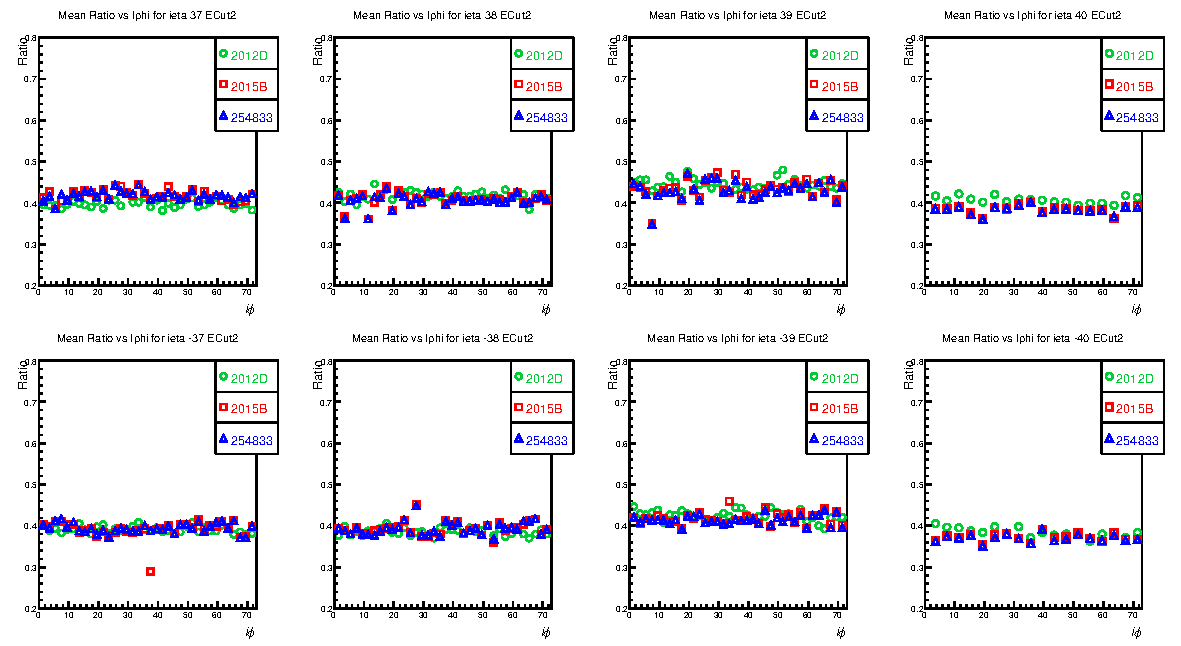
\includegraphics[width=0.99\linewidth]{../Figures/Chap2/ImageFiles_HF/2012vs2015/ieta37to40E1E2Cut2Ietaiphi.pdf}
\caption{\ratiosl vs $i \phi$ for $|i\eta|$ 37 to 40}
\label{fig:ieta37to40E1E2Cut2Ietaiphi}
\end{figure}
\begin{figure}[h!]
\centering
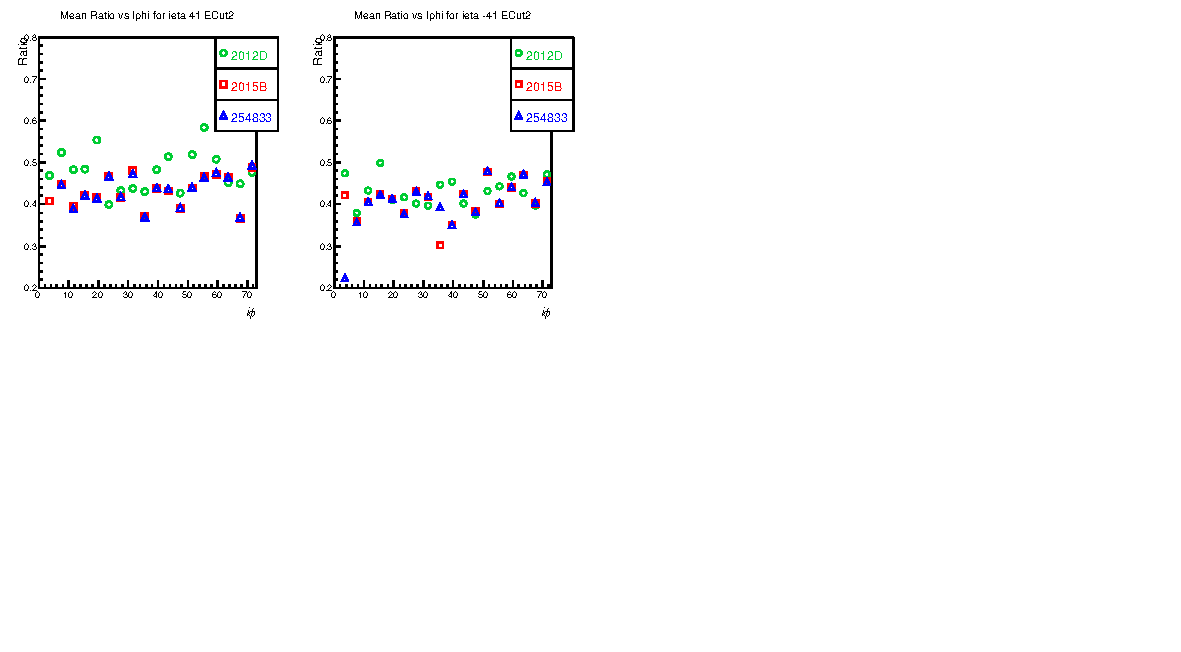
\includegraphics[width=0.99\linewidth]{../Figures/Chap2/ImageFiles_HF/2012vs2015/ieta41E1E2Cut2Ietaiphi.pdf}
\caption{\ratiosl vs $i \phi$ for $|i\eta|$ 41}
\label{fig:ieta41E1E2Cut2Ietaiphi}
\end{figure}

\begin{figure}[h!]
\centering
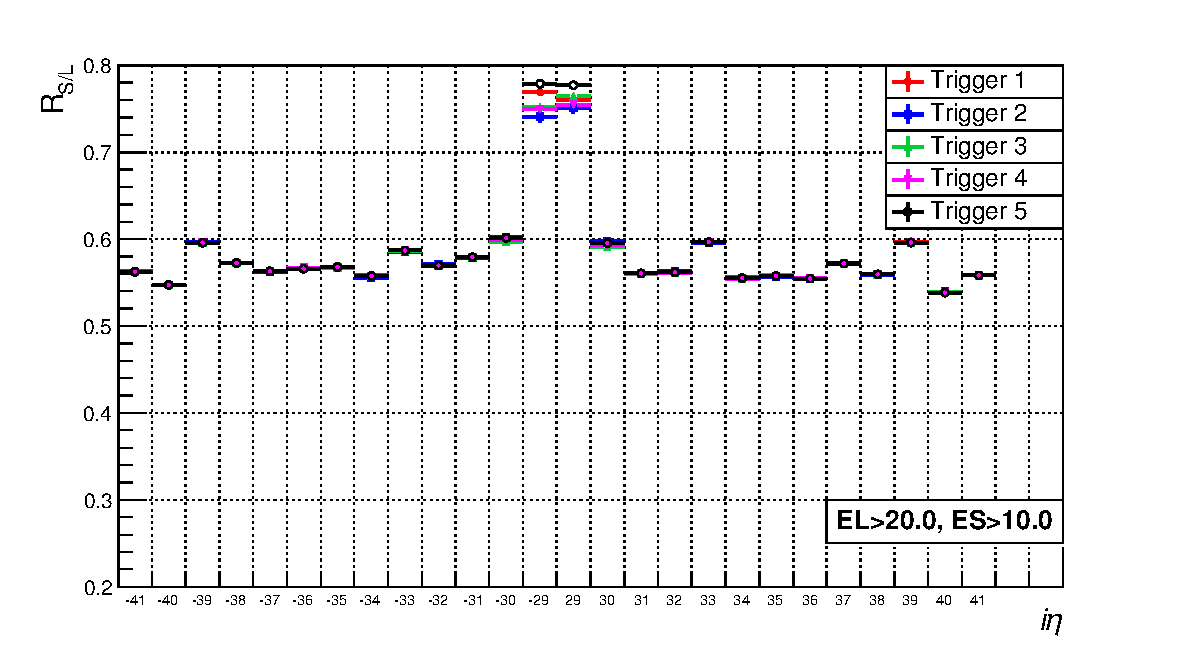
\includegraphics[width=0.99\linewidth]{../Figures/Chap2/ImageFiles_HF/Ratio/2015vs2016/2015DRvsIetaTriggers}
\caption{\ratiosl vs $i \eta$ for 2015D using different triggers 1. HLT\_CaloJet500\_NoJetID, 2. HLT\_DiPFJetAve500, 3. HLT\_PFHT750\_4JetPt50, 4. HLT\_PFHT800, 5. HLT\_PFJet450}
\label{2015DRvsIetaTriggers}
\end{figure}


% % % % % % % % % % % % % % % % % % % % % % % %
%             2016 Data
% % % % % % % % % % % % % % % % % % % % % % % %

\clearpage
\begin{figure}
\centering
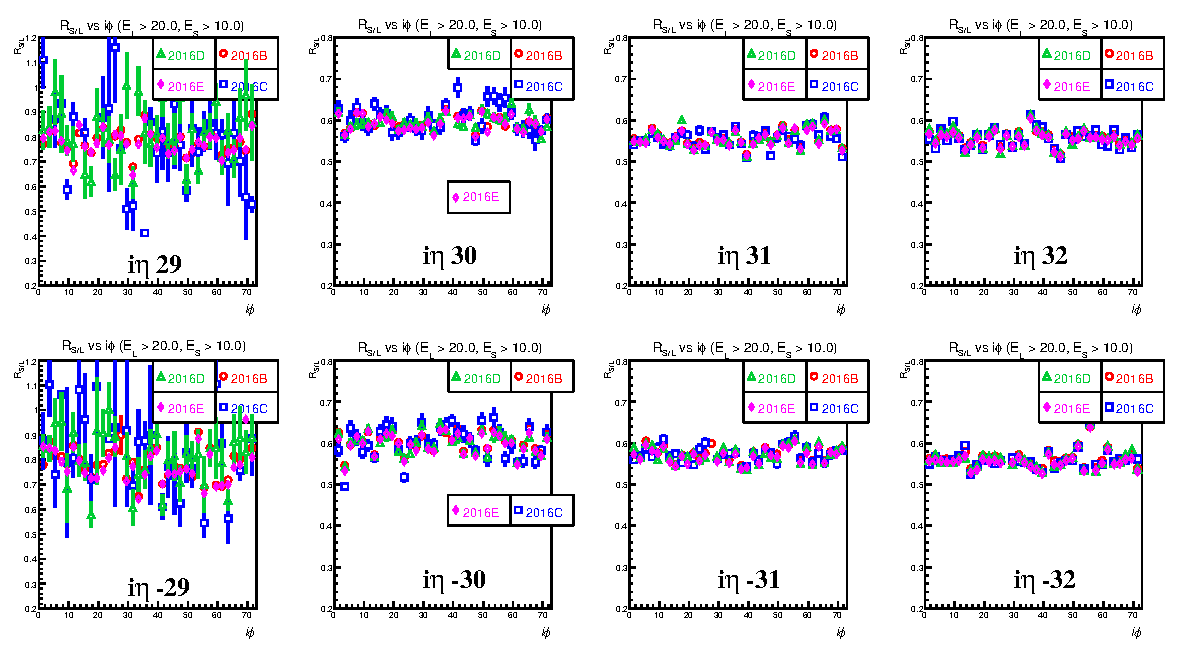
\includegraphics[width=0.99\linewidth]{../Figures/Chap2/ImageFiles_HF/Ratio/2016/RvsIphi2016BtoE/ieta29_32_E1E2Cut0Ietaiphi}
\caption{\ratiosl as a function of $i\phi$ for $|i\eta|$ 29 to 32 for 2016BtoE}
\label{fig:ieta29_32_E1E2Cut0Ietaiphi2016BtoE}
\end{figure}
\begin{figure}
\centering
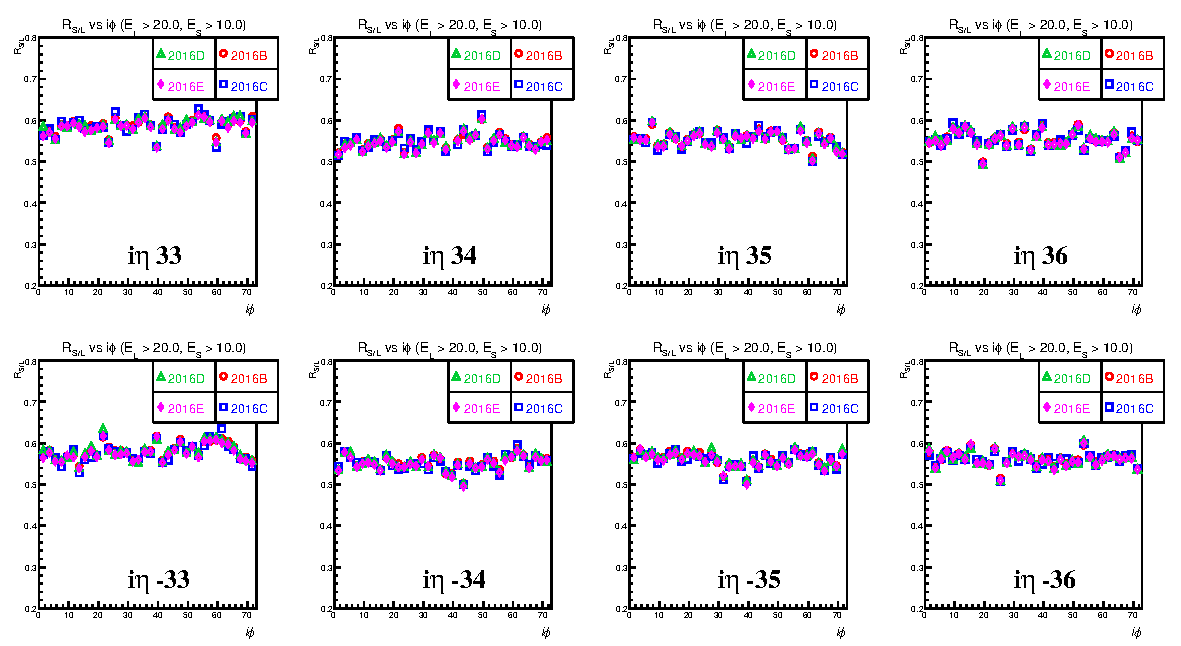
\includegraphics[width=0.99\linewidth]{../Figures/Chap2/ImageFiles_HF/Ratio/2016/RvsIphi2016BtoE/ieta33_36_E1E2Cut0Ietaiphi}
\caption{\ratiosl as a function of $i\phi$ for $|i\eta|$ 33 to 36 for 2016BtoE}
\label{fig:ieta33_36_E1E2Cut0Ietaiphi2016BtoE}
\end{figure}
\begin{figure}
\centering
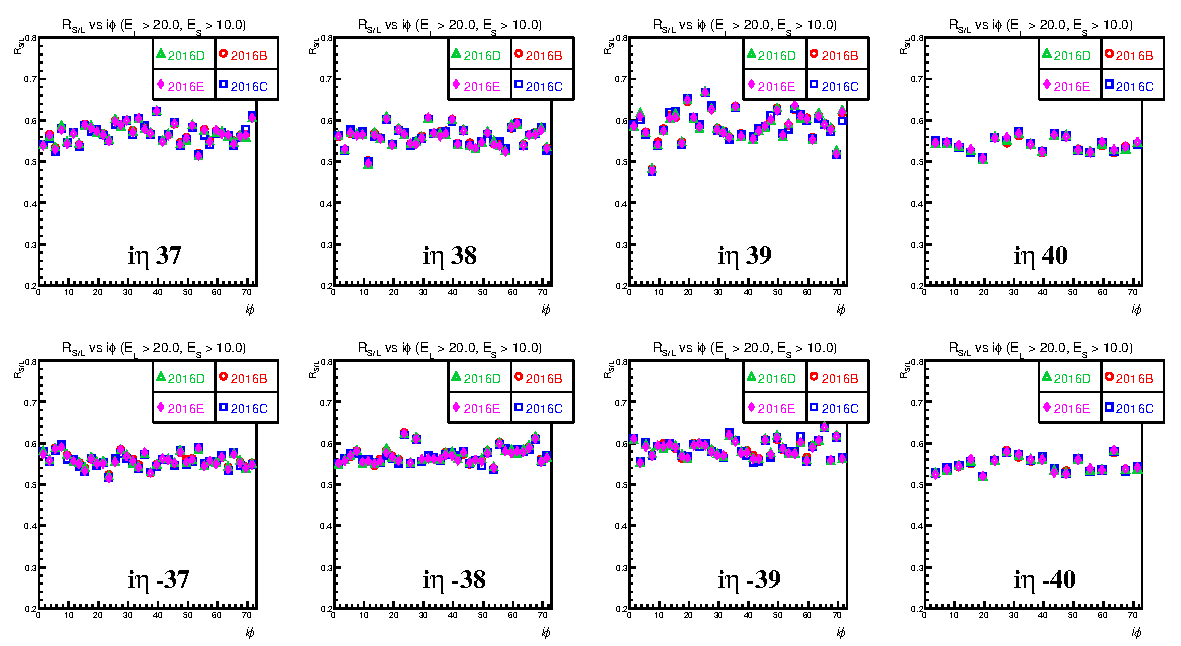
\includegraphics[width=0.99\linewidth]{../Figures/Chap2/ImageFiles_HF/Ratio/2016/RvsIphi2016BtoE/ieta37_40_E1E2Cut0Ietaiphi}
\caption{\ratiosl as a function of $i\phi$ for $|i\eta|$ 37 to 40 for 2016BtoE}
\label{fig:ieta37_40_E1E2Cut0Ietaiphi2016BtoE}
\end{figure}
\begin{figure}
\centering
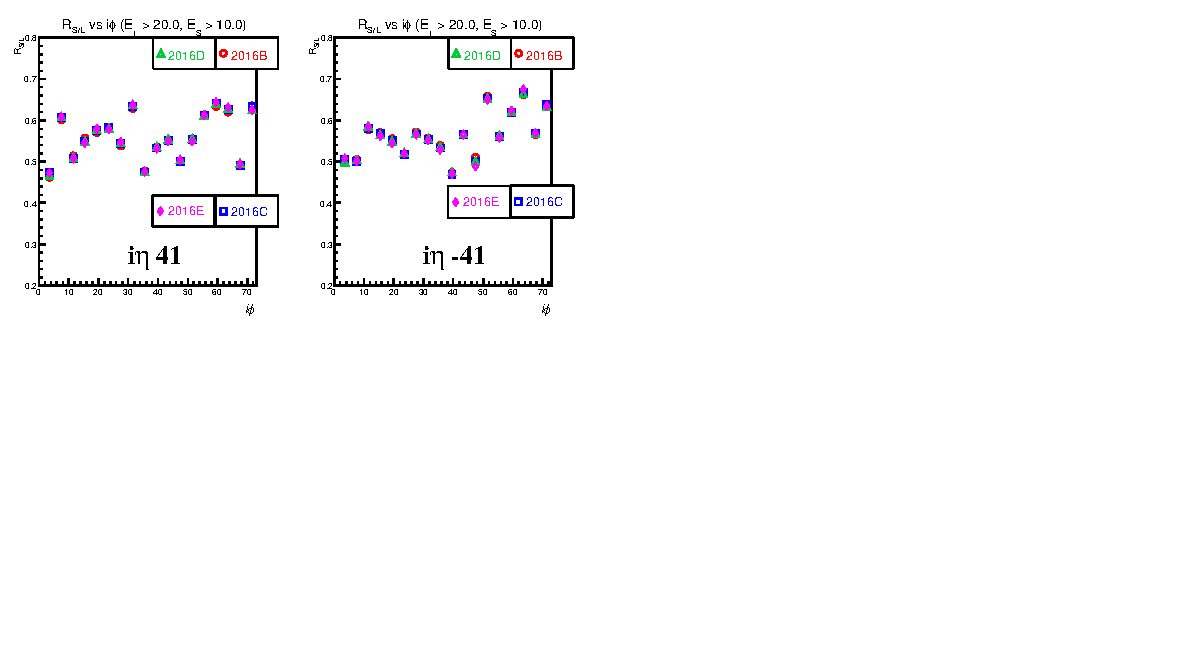
\includegraphics[width=0.99\linewidth]{../Figures/Chap2/ImageFiles_HF/Ratio/2016/RvsIphi2016BtoE/ieta41_E1E2Cut0Ietaiphi}
\caption{\ratiosl as a function of $i\phi$ for $|i\eta|$ 41 for 2016BtoE}
\label{fig:ieta41_E1E2Cut0Ietaiphi2016BtoE}
\end{figure}

\begin{figure}[h!]
\centering
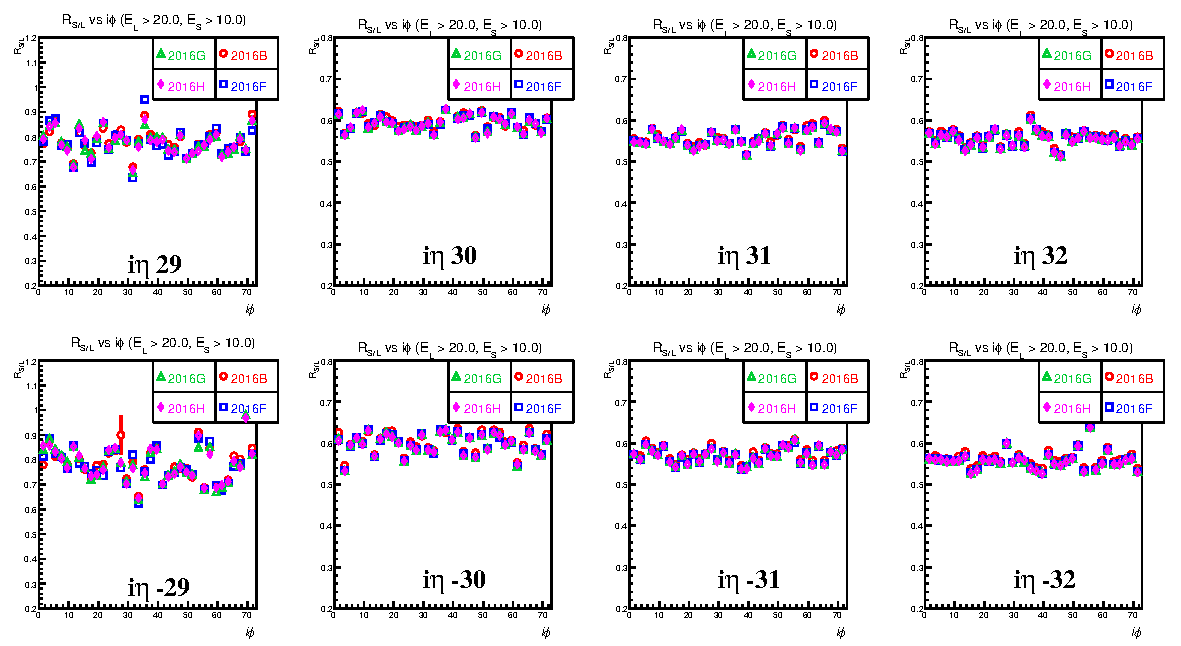
\includegraphics[width=0.99\linewidth]{../Figures/Chap2/ImageFiles_HF/Ratio/2016/RvsIphi2016BFGH/ieta29_32_E1E2Cut0Ietaiphi}
\caption{\ratiosl as a function of $i\phi$ for $|i\eta|$ 29 to 32 for 2016B,F,G,H}
\label{fig:ieta29_32_E1E2Cut0Ietaiphi2016BFGH}
\end{figure}
\begin{figure}[h!]
\centering
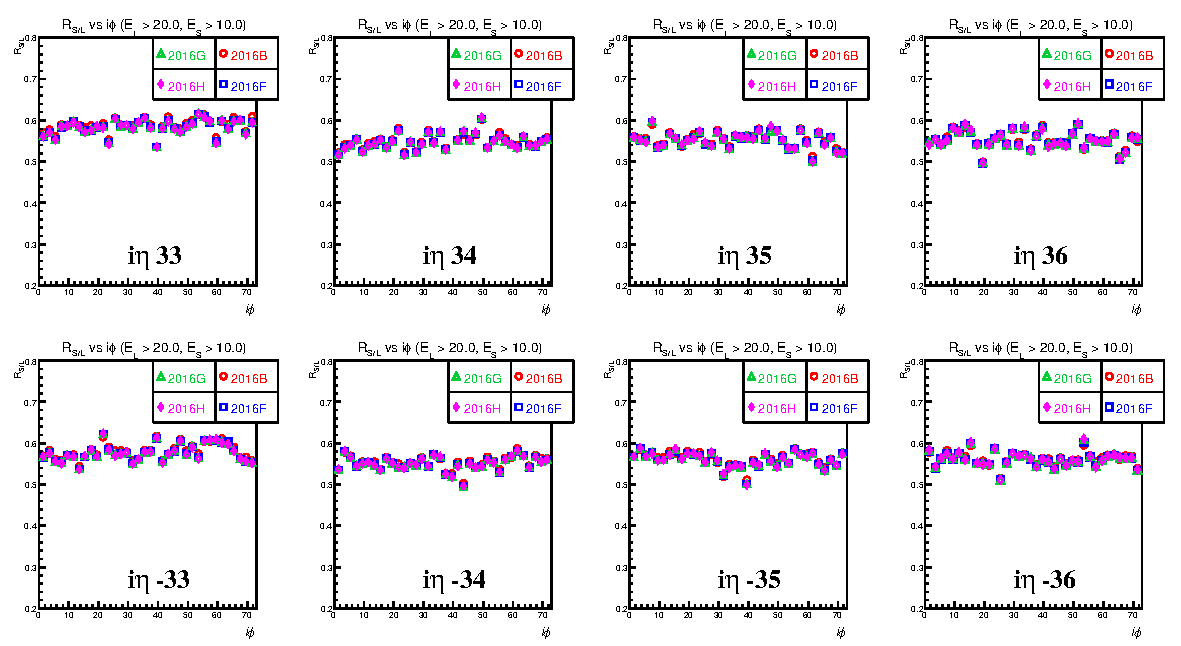
\includegraphics[width=0.99\linewidth]{../Figures/Chap2/ImageFiles_HF/Ratio/2016/RvsIphi2016BFGH/ieta33_36_E1E2Cut0Ietaiphi}
\caption{\ratiosl as a function of $i\phi$ for $|i\eta|$ 33 to 36 for 2016B,F,G,H}
\label{fig:ieta33_36_E1E2Cut0Ietaiphi2016BFGH}
\end{figure}
\begin{figure}[h!]
\centering
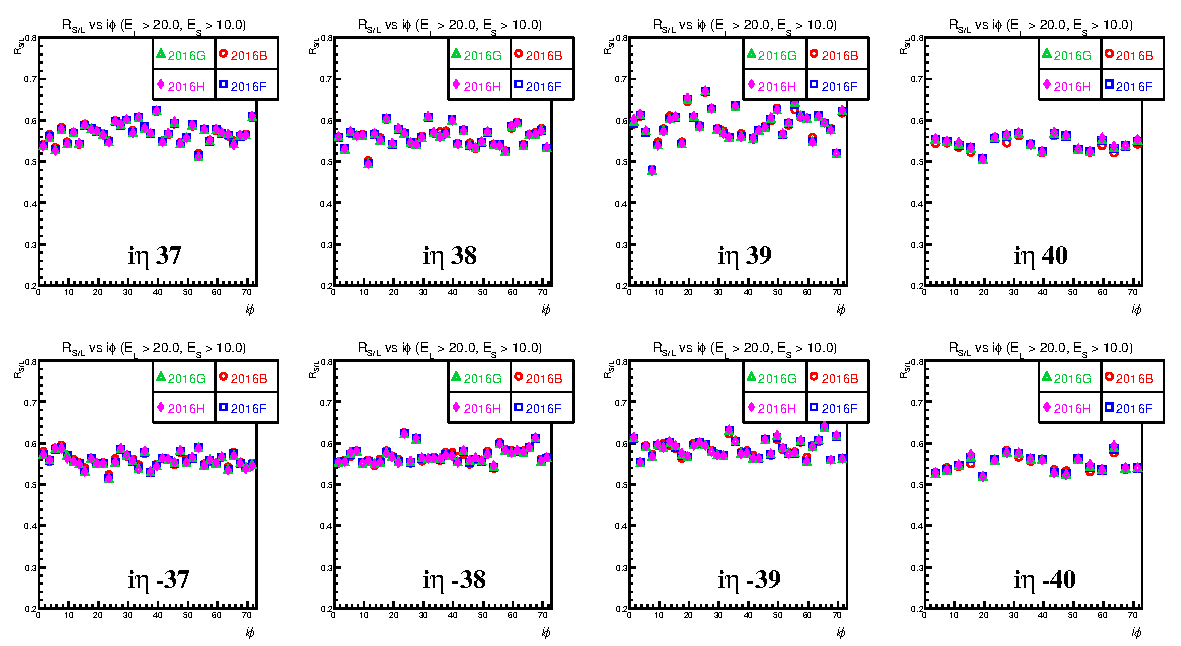
\includegraphics[width=0.99\linewidth]{../Figures/Chap2/ImageFiles_HF/Ratio/2016/RvsIphi2016BFGH/ieta37_40_E1E2Cut0Ietaiphi}
\caption{\ratiosl as a function of $i\phi$ for $|i\eta|$ 37 to 40 for 2016B,F,G,H}
\label{fig:ieta37_40_E1E2Cut0Ietaiphi2016BFGH}
\end{figure}
\begin{figure}[h!]
\centering
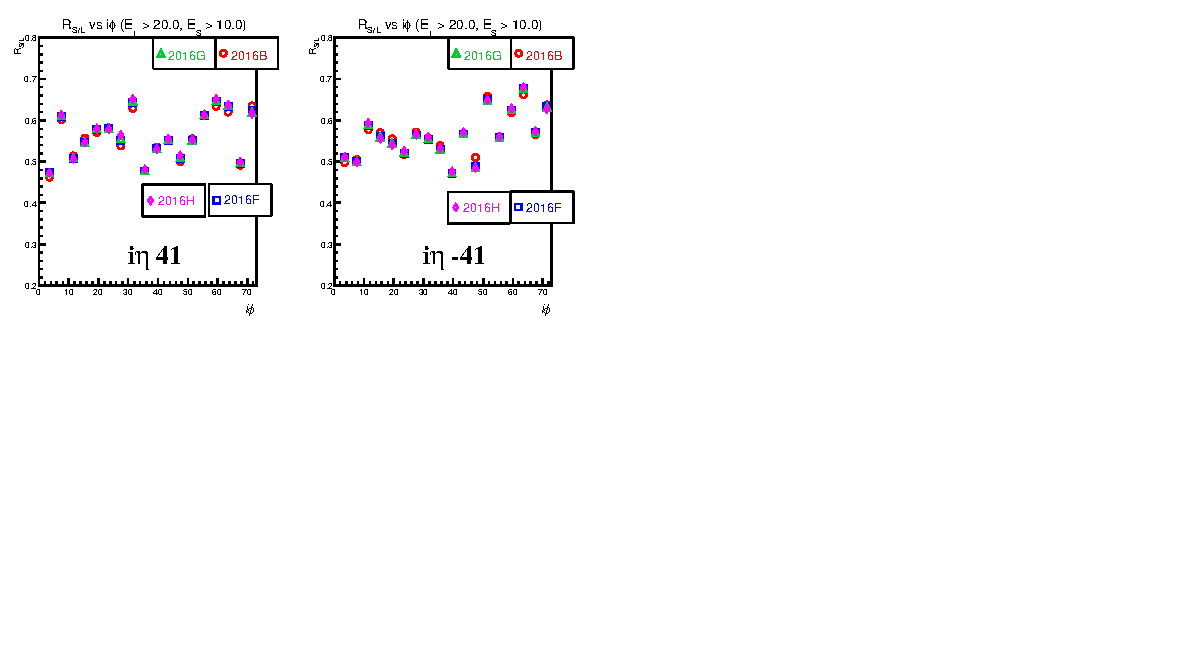
\includegraphics[width=0.99\linewidth]{../Figures/Chap2/ImageFiles_HF/Ratio/2016/RvsIphi2016BFGH/ieta41_E1E2Cut0Ietaiphi}
\caption{\ratiosl as a function of $i\phi$ for $|i\eta|$ 41 for 2016B,F,G,H}
\label{fig:ieta41_E1E2Cut0Ietaiphi2016BFGH}
\end{figure}

\begin{figure}[h!]
\centering
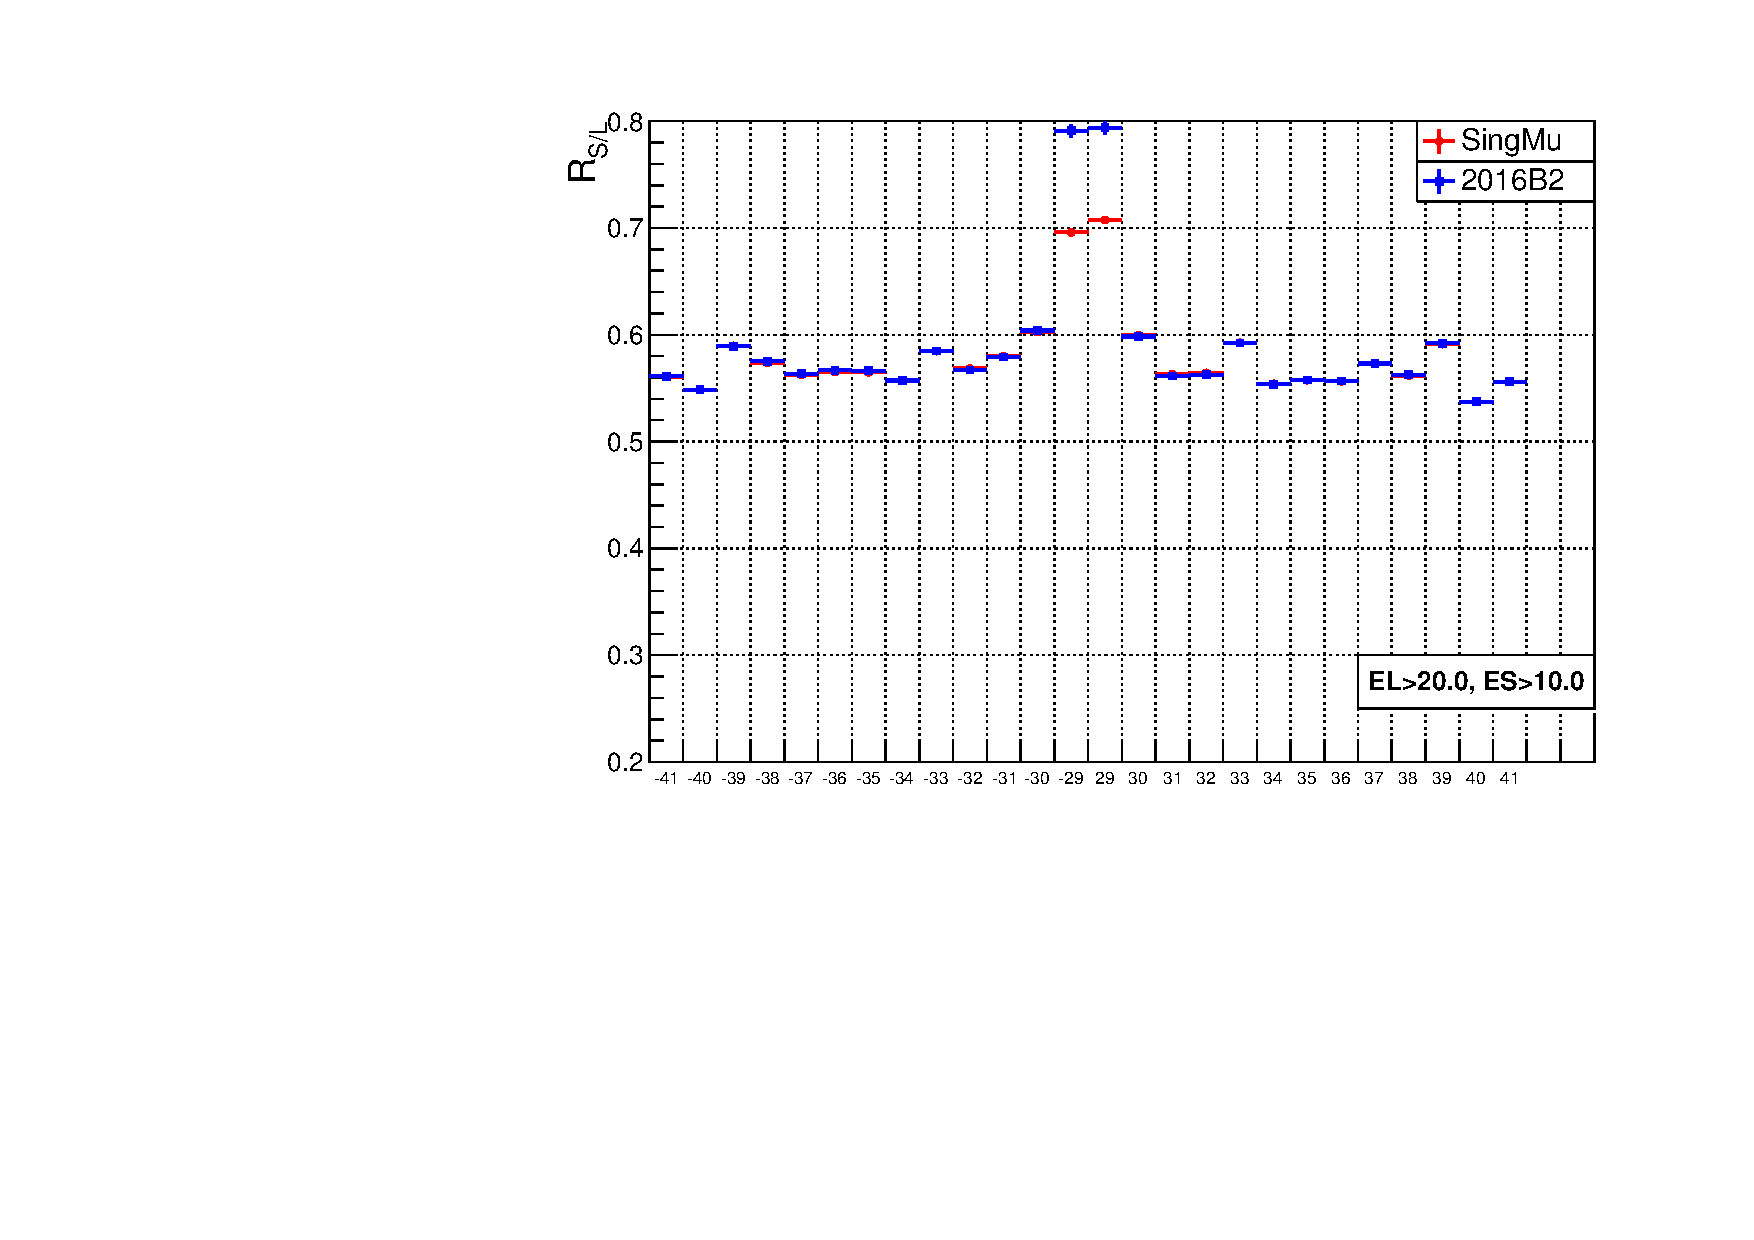
\includegraphics[width=0.99\linewidth]{../Figures/Chap2/ImageFiles_HF/Ratio/2016/2016B2SingMu}
\caption{\ratiosl as a function of $i\eta$ for 2016B using JetHT(labelled as 2016B2 in blue) and SingleMuon datasets. Runs used:
273448,273492-273728.}
\label{fig:2016B2SingMu}
\end{figure}

% % % % % % % % % % % % % % % % % % % % % % % %
%             2016 Correction
% % % % % % % % % % % % % % % % % % % % % % % %
%			BtoE
\clearpage
\begin{figure}[h!]
\centering
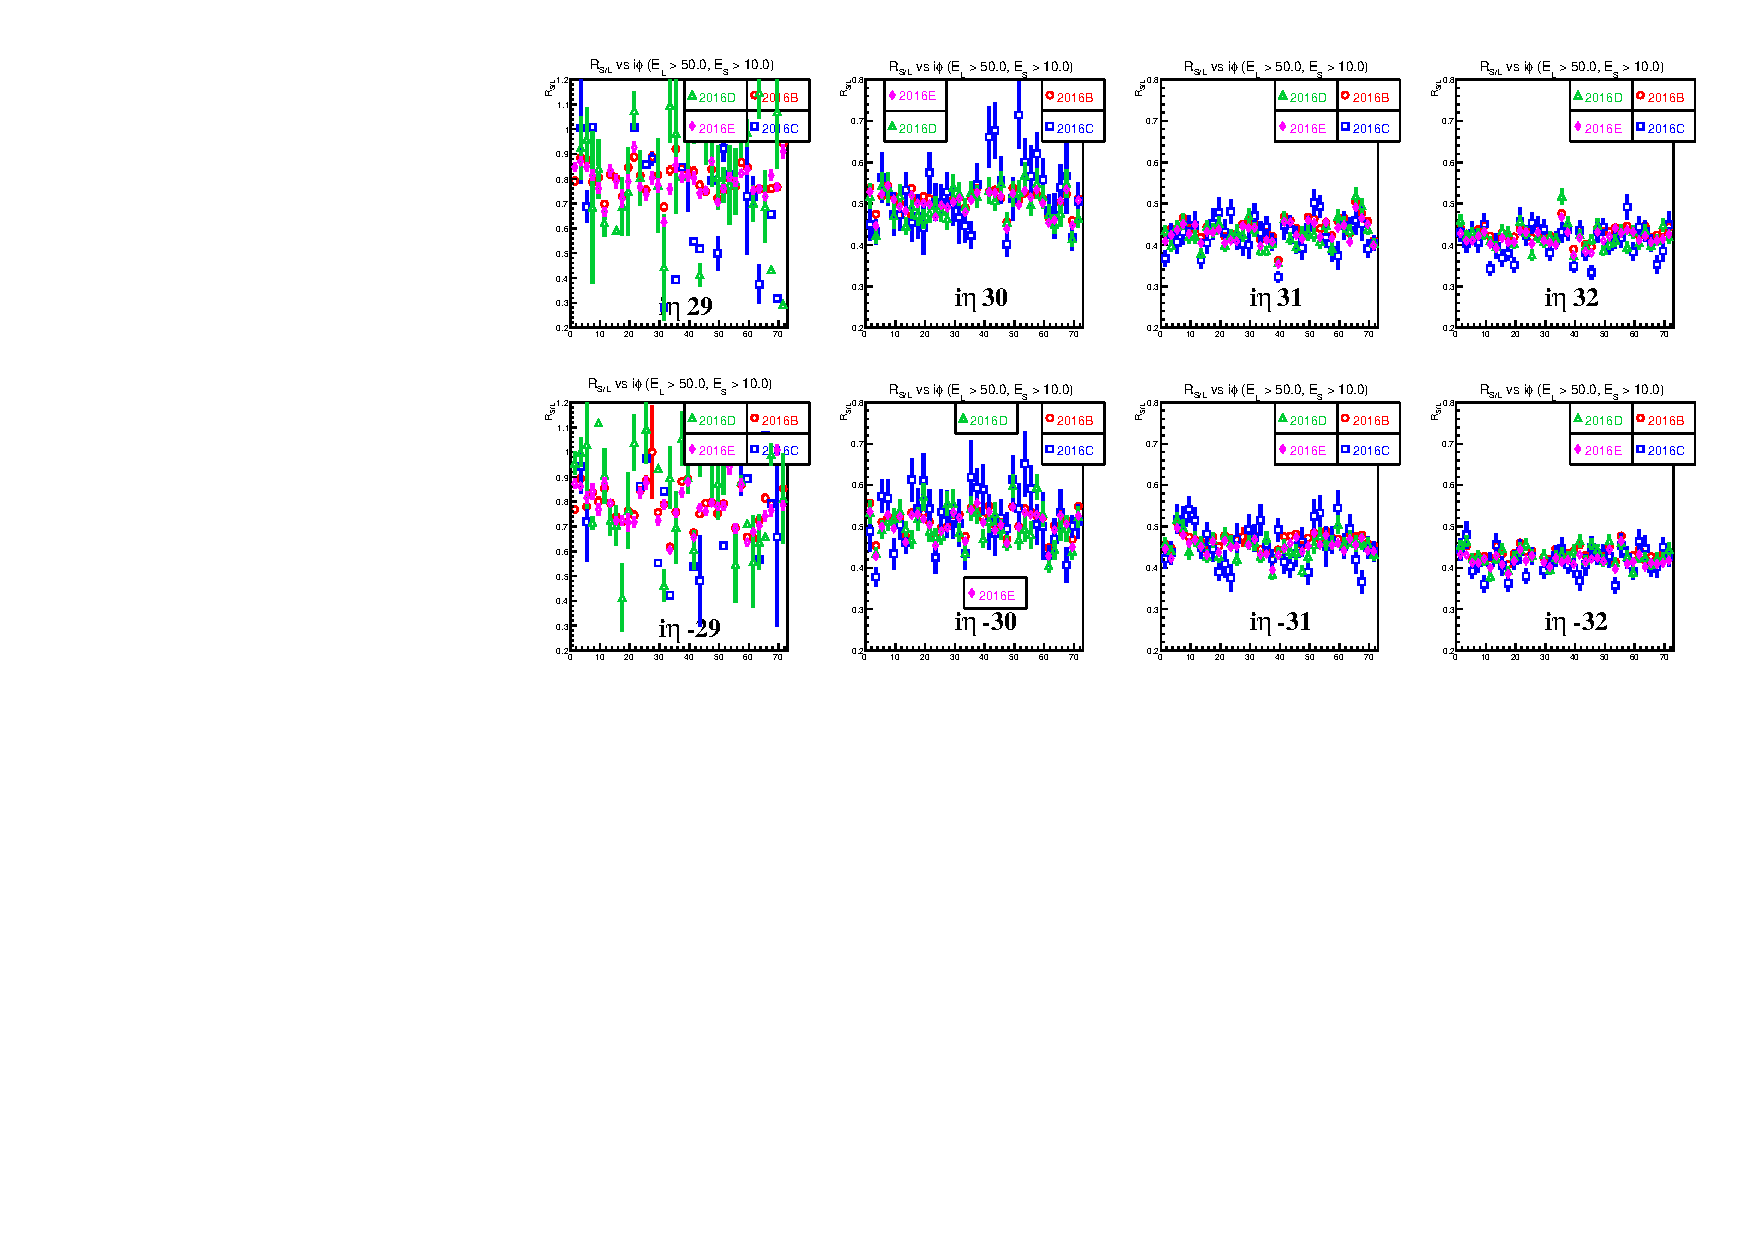
\includegraphics[width=0.99\linewidth]{../Figures/Chap2/ImageFiles_HF/Ratio/2016/Corrected/2016BtoE/ieta29_32_E1E2Cut3Ietaiphi}
\caption{\ratiosl vs $i\phi$ for $|i\eta|$ 29 to 32 for 2016BtoE(Correction NOT applied)}
\label{fig:ieta29_32_E1E2Cut3IetaiphiBtoE}
\end{figure}
\begin{figure}[h!]
\centering
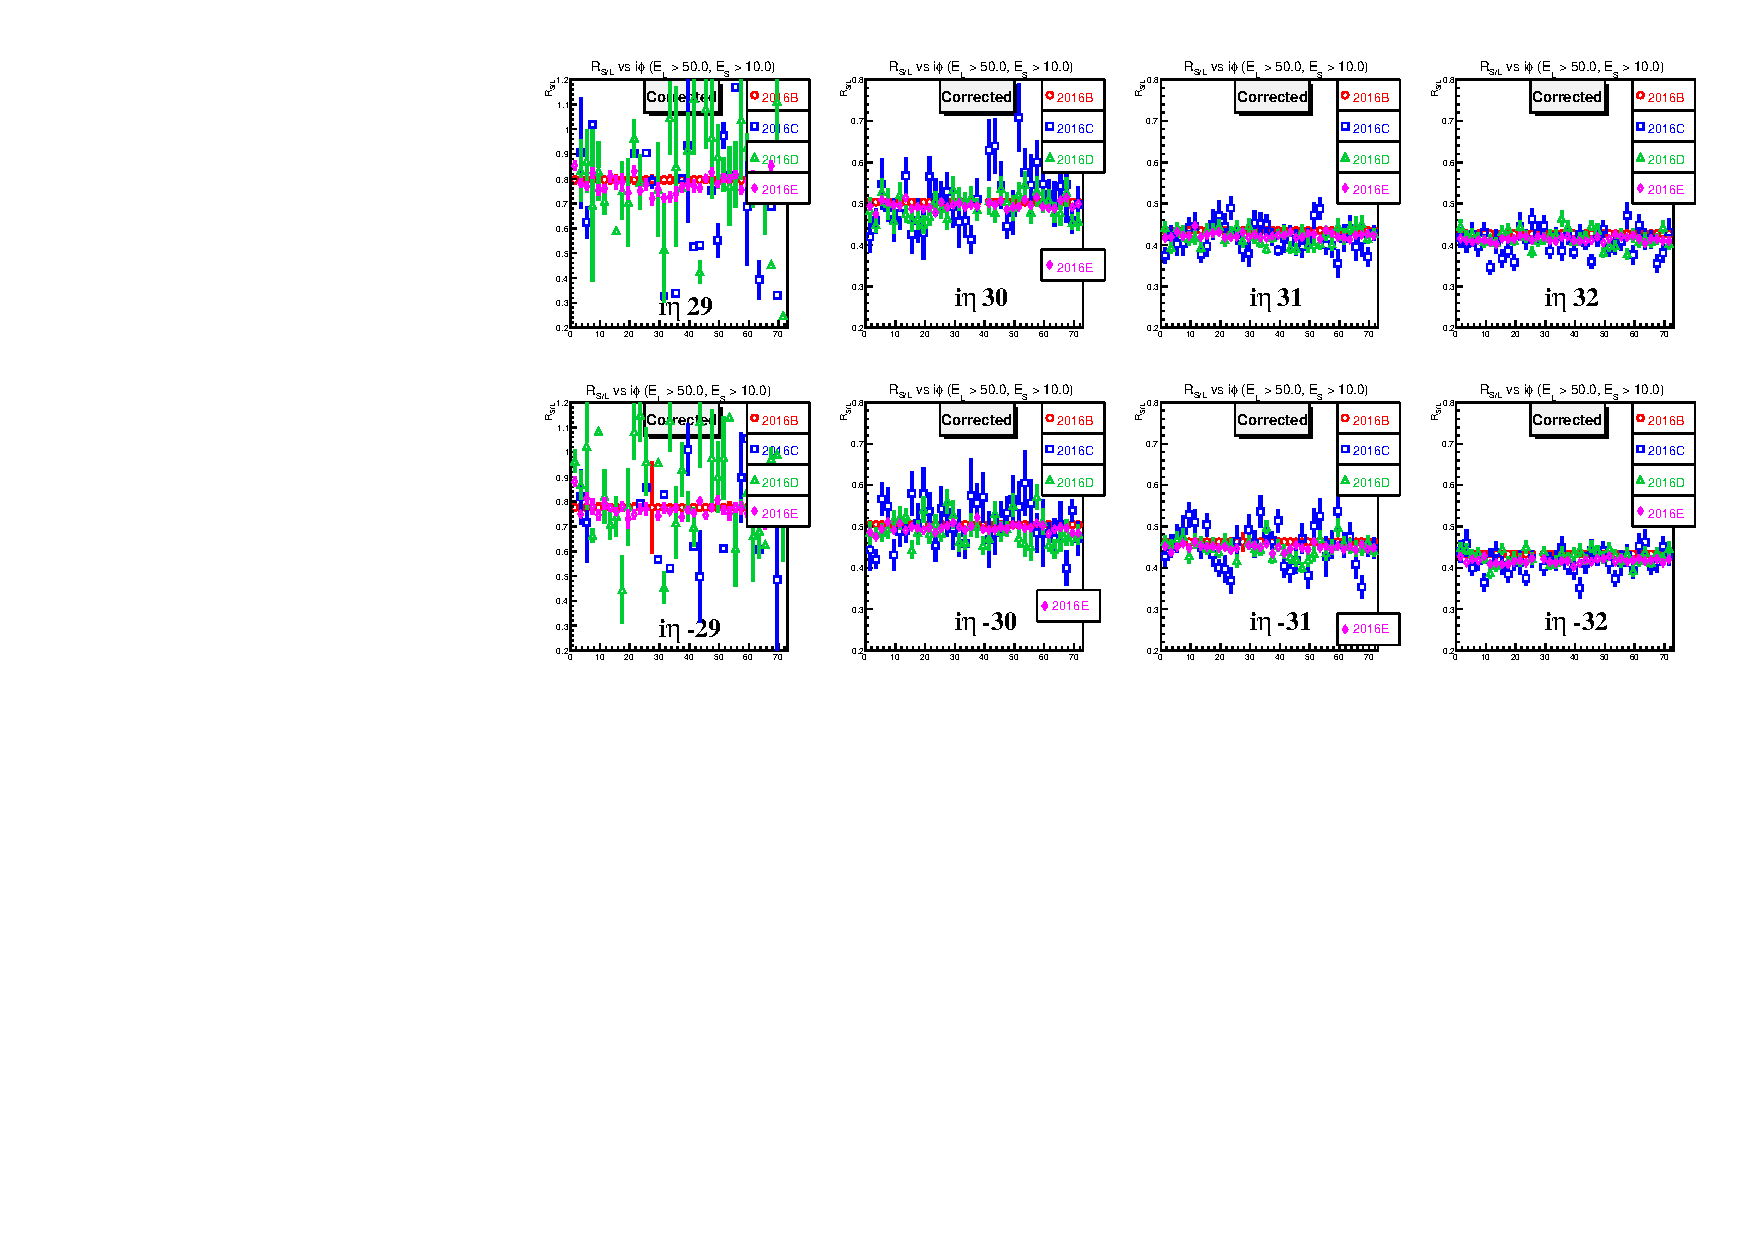
\includegraphics[width=0.99\linewidth]{../Figures/Chap2/ImageFiles_HF/Ratio/2016/Corrected/2016BtoE/ieta29_32_E1E2Cut3Ietaiphi_Crrtd}
\caption{\ratiosl vs $i\phi$ for $|i\eta|$ 29 to 32 for 2016BtoE(Correction applied)}
\label{fig:ieta29_32_E1E2Cut3Ietaiphi_CrrtdBtoE}
\end{figure}
\newpage
\begin{figure}[h!]
\centering
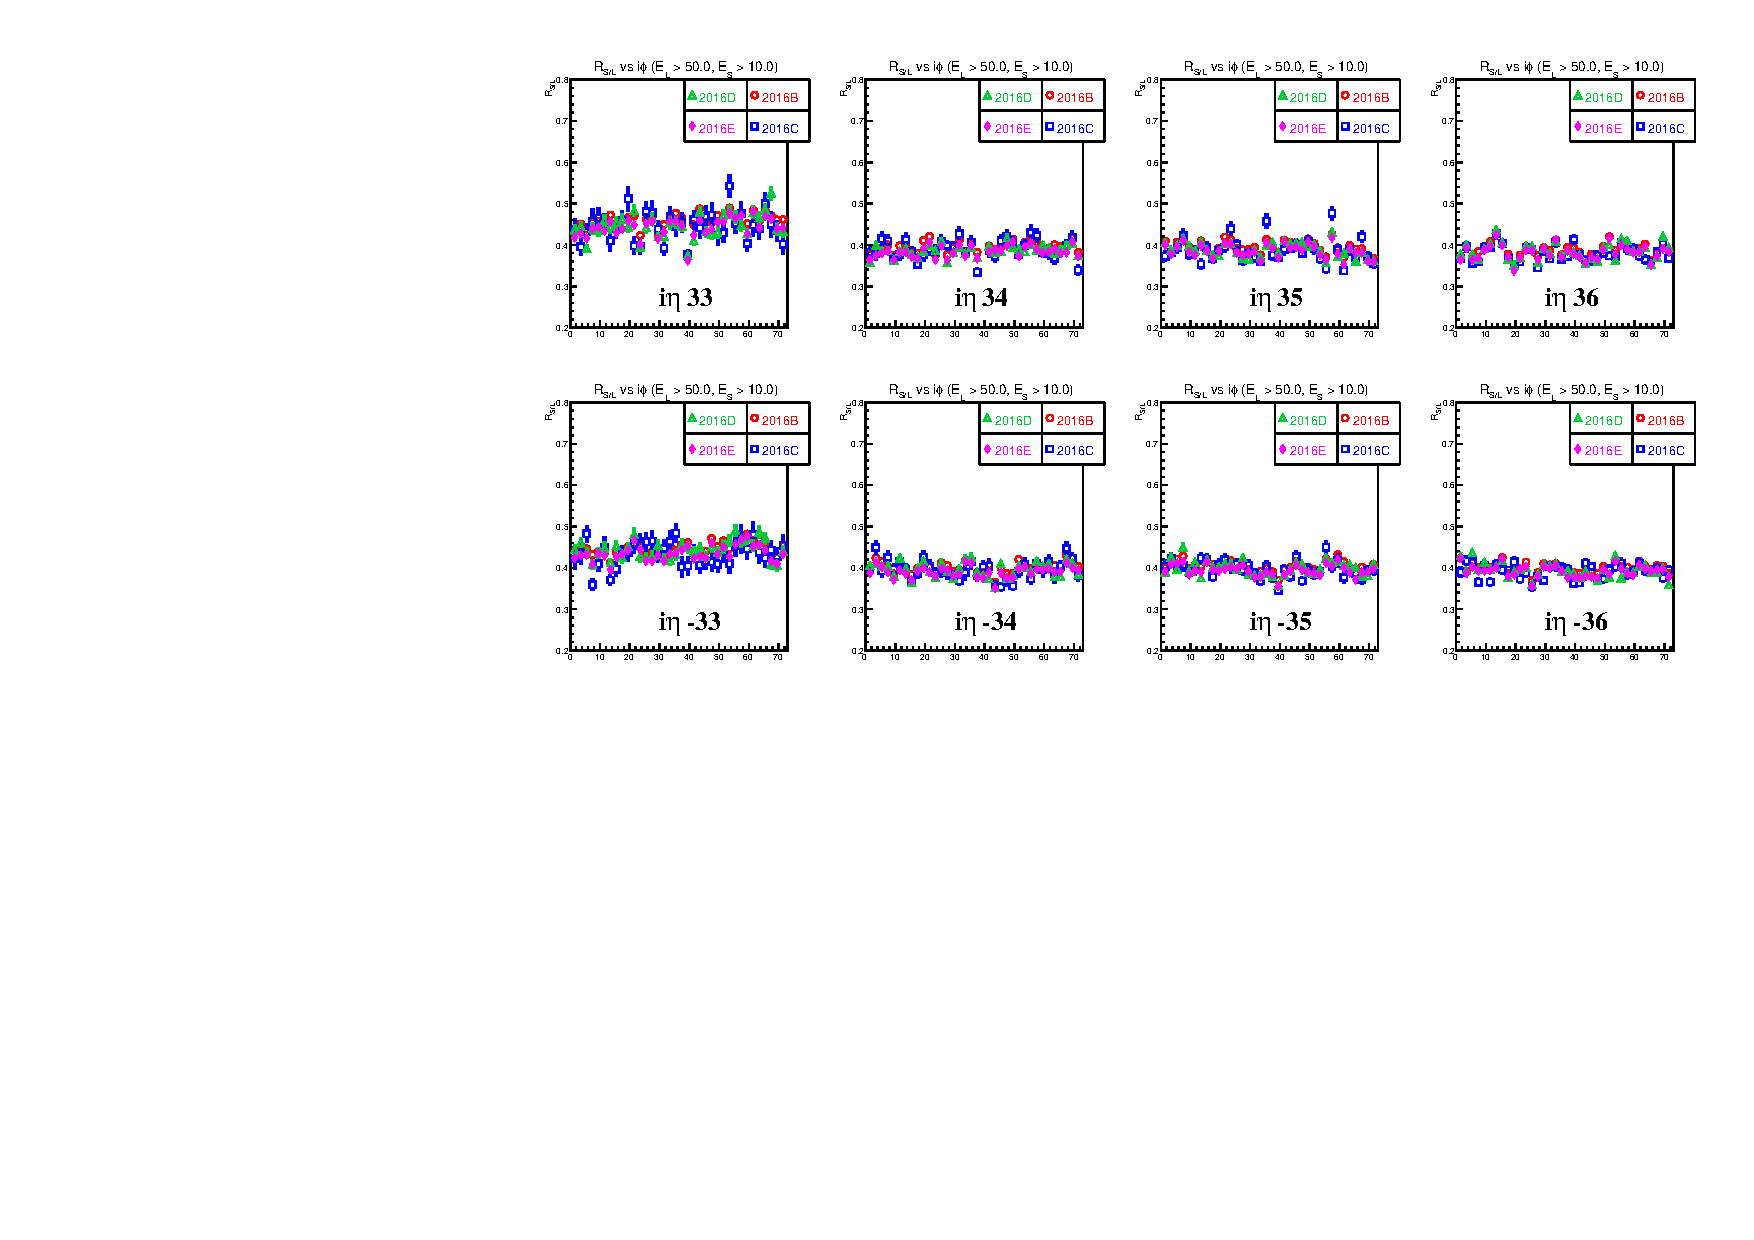
\includegraphics[width=0.99\linewidth]{../Figures/Chap2/ImageFiles_HF/Ratio/2016/Corrected/2016BtoE/ieta33_36_E1E2Cut3Ietaiphi}
\caption{\ratiosl vs $i\phi$ for $|i\eta|$ 33 to 36 for 2016BtoE(Correction NOT applied)}
\label{fig:ieta33_36_E1E2Cut3IetaiphiBtoE}
\end{figure}
\begin{figure}[h!]
\centering
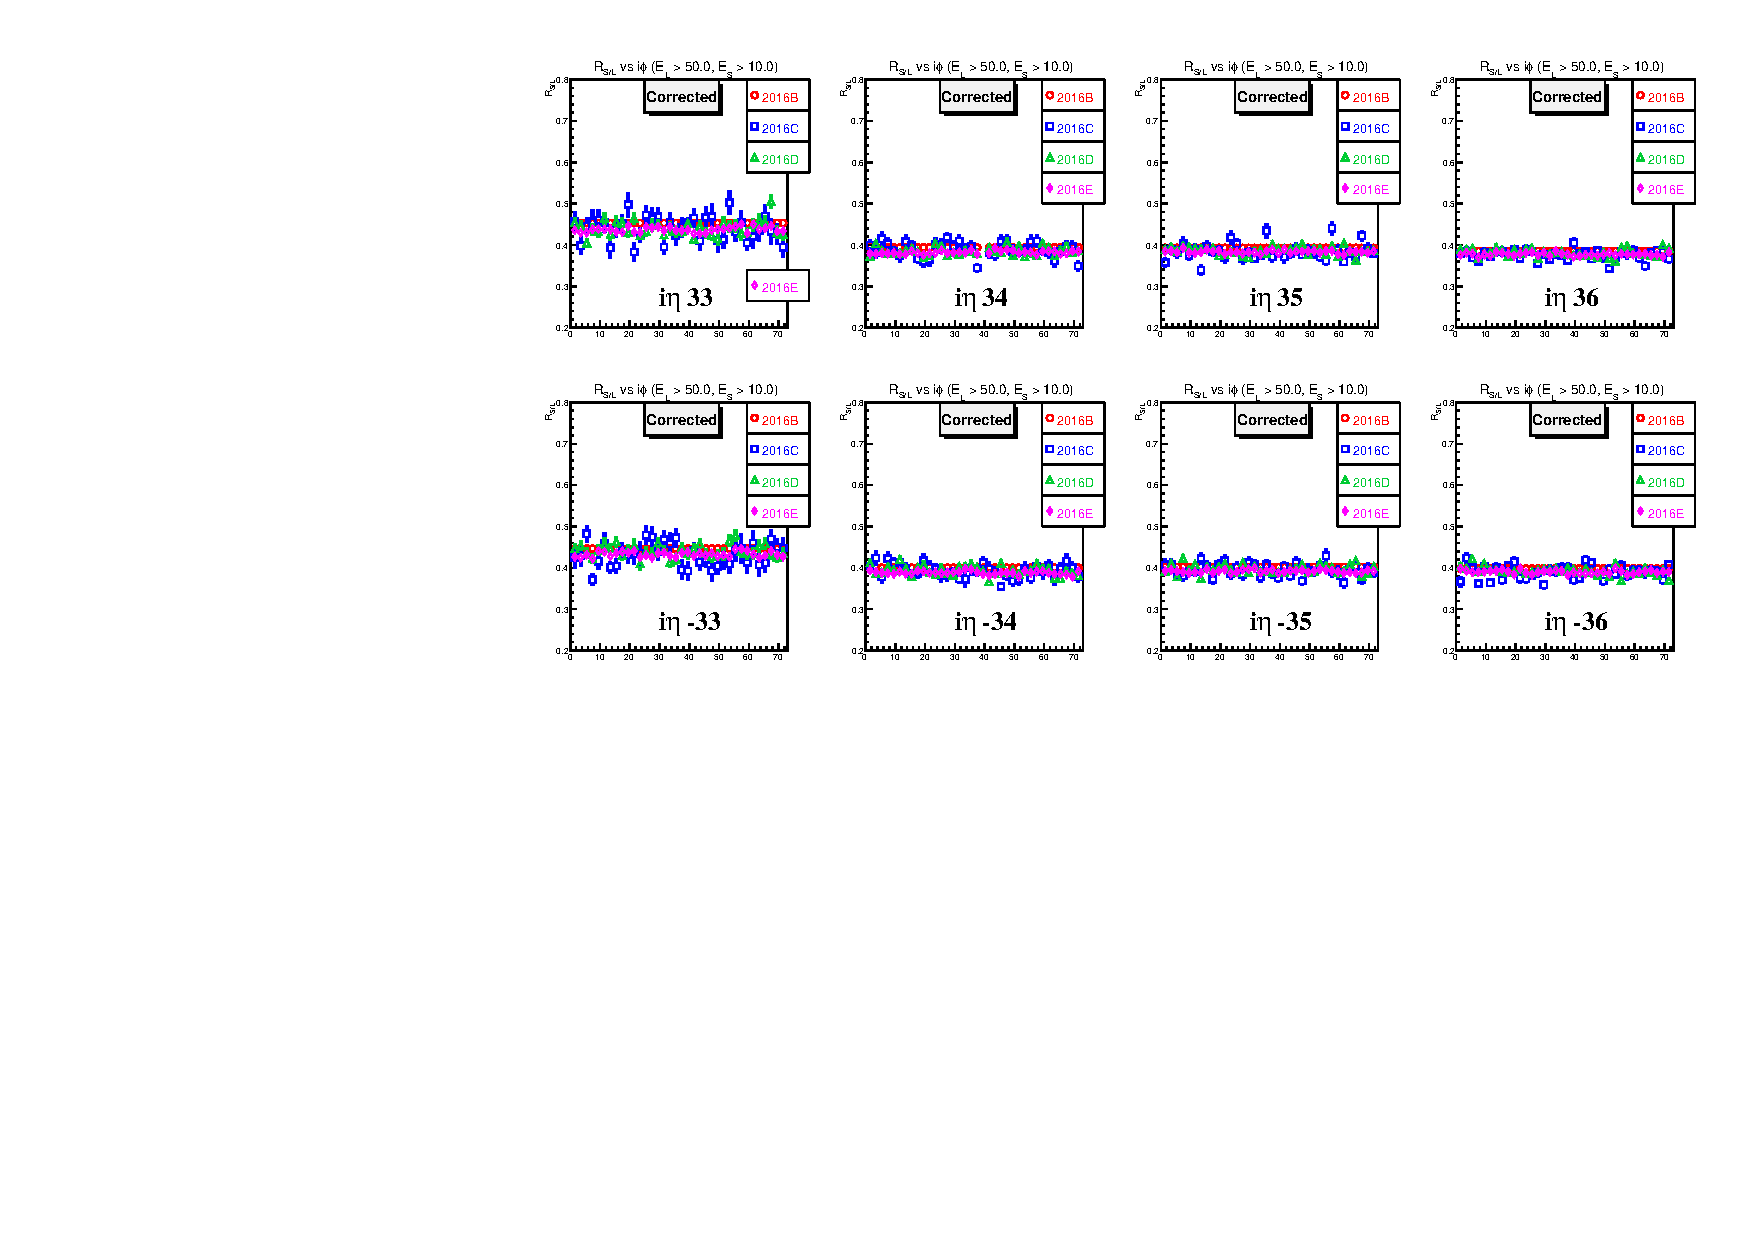
\includegraphics[width=0.99\linewidth]{../Figures/Chap2/ImageFiles_HF/Ratio/2016/Corrected/2016BtoE/ieta33_36_E1E2Cut3Ietaiphi_Crrtd}
\caption{\ratiosl vs $i\phi$ for $|i\eta|$ 33 to 36 for 2016BtoE(Correction applied)}
\label{fig:ieta33_36_E1E2Cut3Ietaiphi_CrrtdBtoE}
\end{figure}
\newpage
\begin{figure}[h!]
\centering
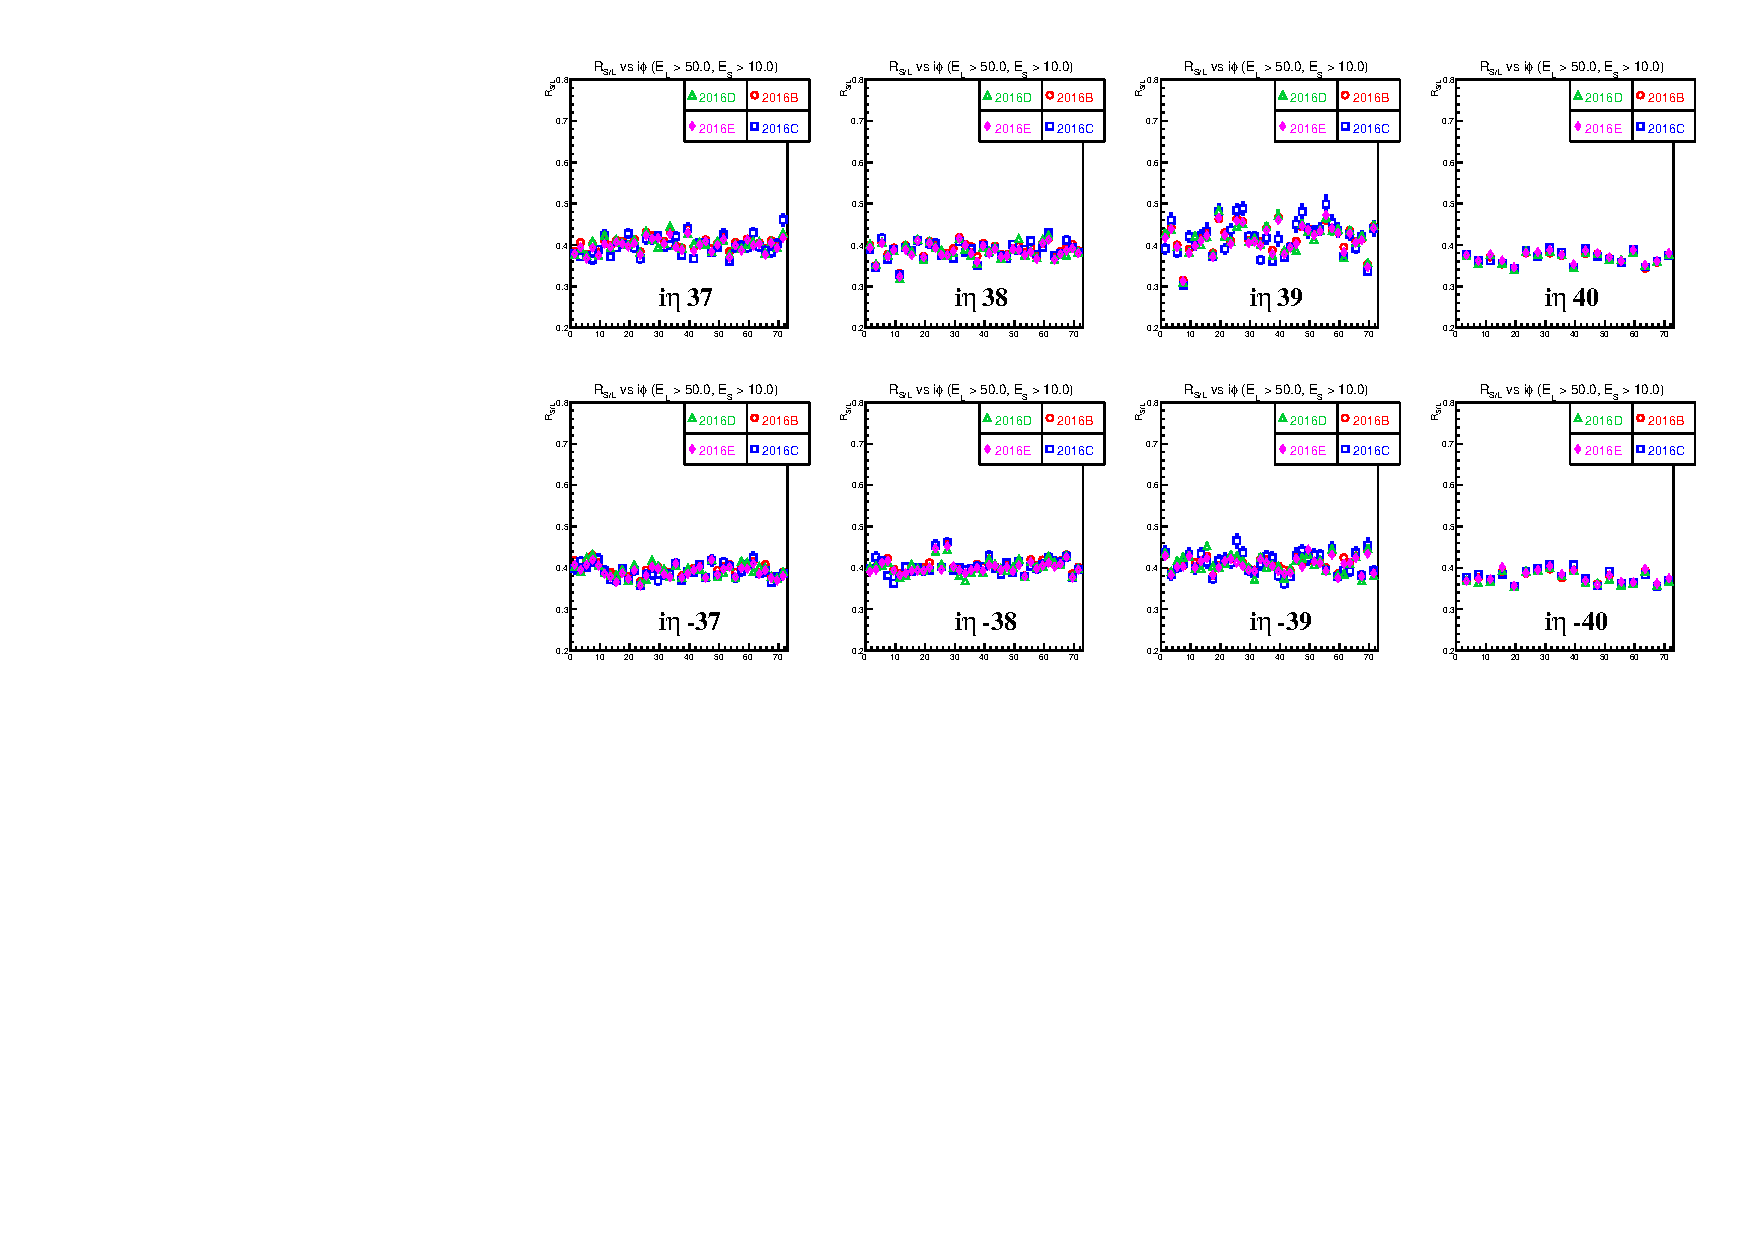
\includegraphics[width=0.99\linewidth]{../Figures/Chap2/ImageFiles_HF/Ratio/2016/Corrected/2016BtoE/ieta37_40_E1E2Cut3Ietaiphi}
\caption{\ratiosl vs $i\phi$ for $|i\eta|$ 37 to 40 for 2016BtoE(Correction NOT applied)}
\label{fig:ieta37_40_E1E2Cut3IetaiphiBtoE}
\end{figure}
\begin{figure}[h!]
\centering
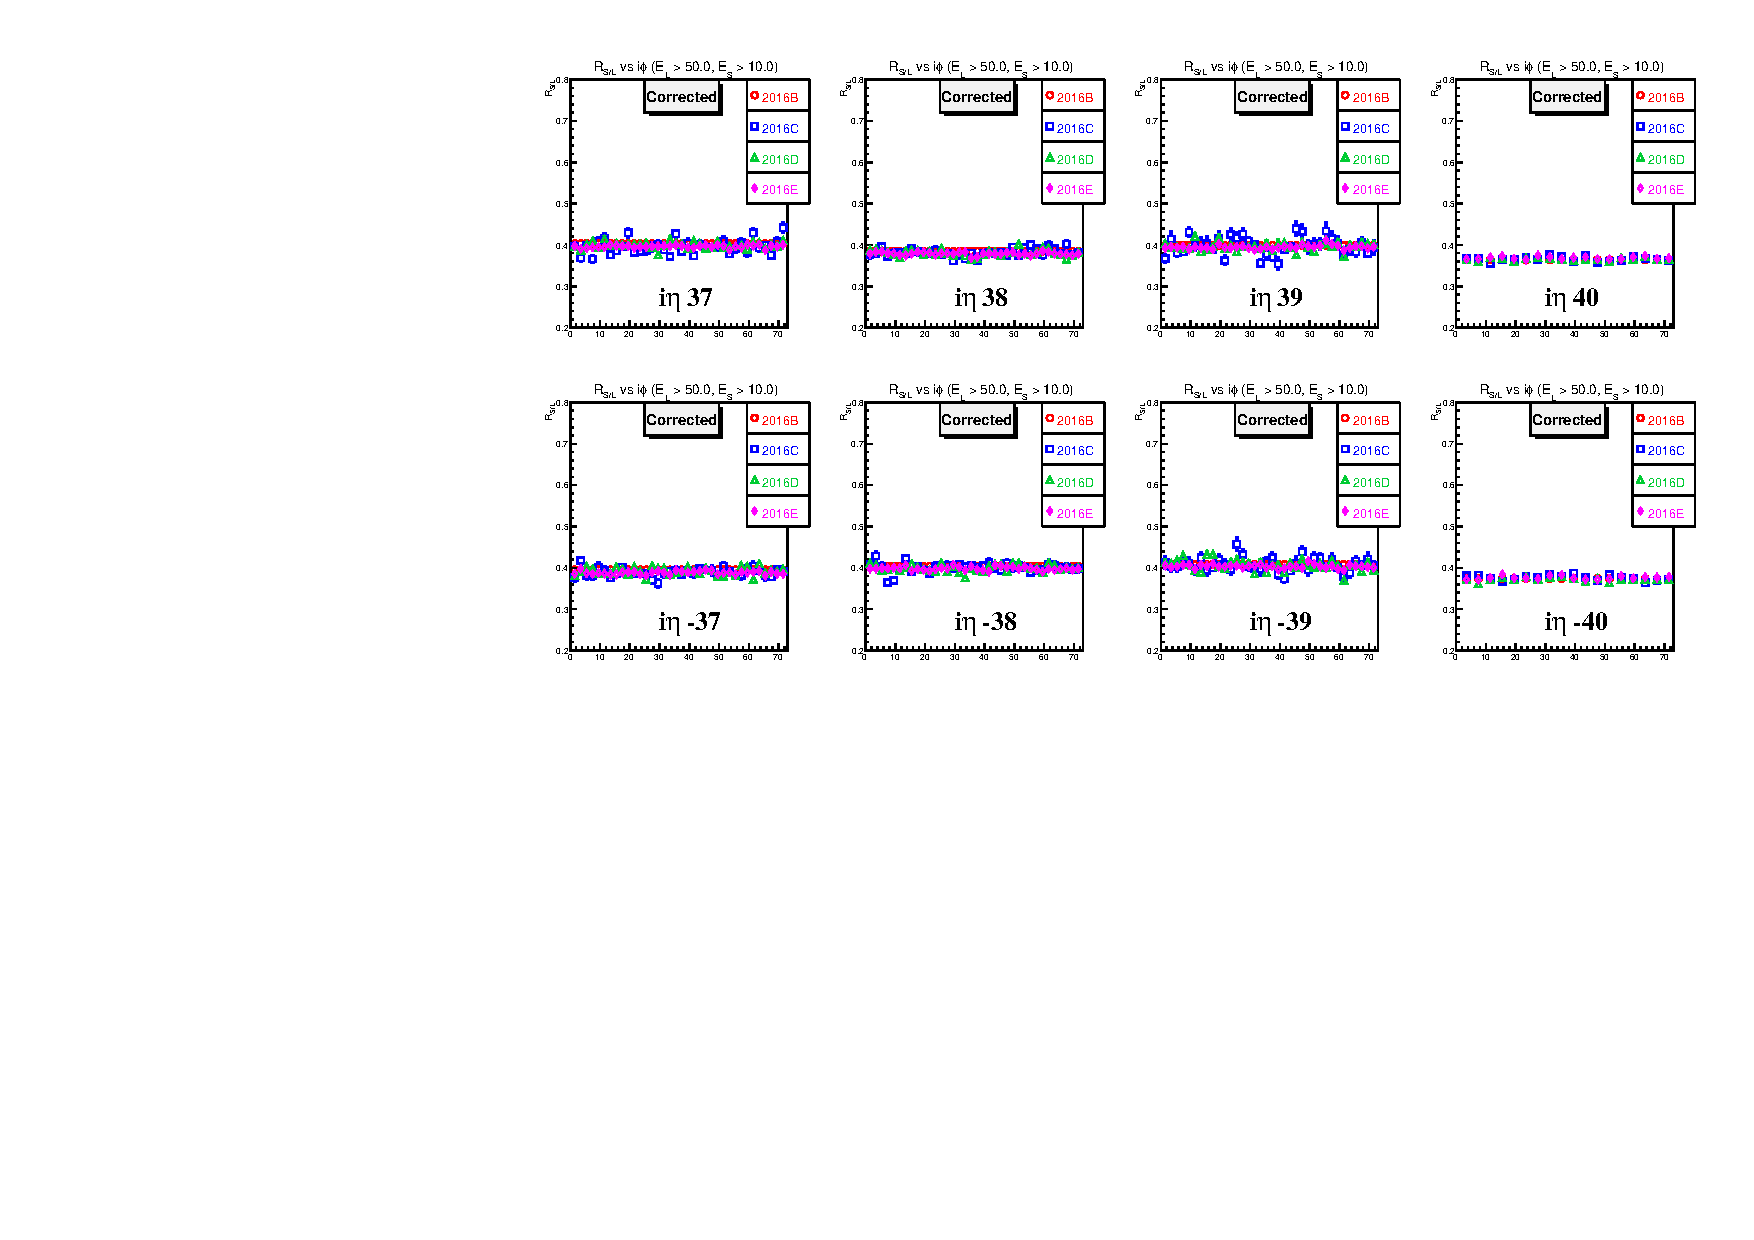
\includegraphics[width=0.99\linewidth]{../Figures/Chap2/ImageFiles_HF/Ratio/2016/Corrected/2016BtoE/ieta37_40_E1E2Cut3Ietaiphi_Crrtd}
\caption{\ratiosl vs $i\phi$ for $|i\eta|$ 33 to 36 for 2016BtoE(Correction applied)}
\label{fig:ieta37_40_E1E2Cut3Ietaiphi_CrrtdBtoE}
\end{figure}
\newpage
\begin{figure}[h!]
\centering
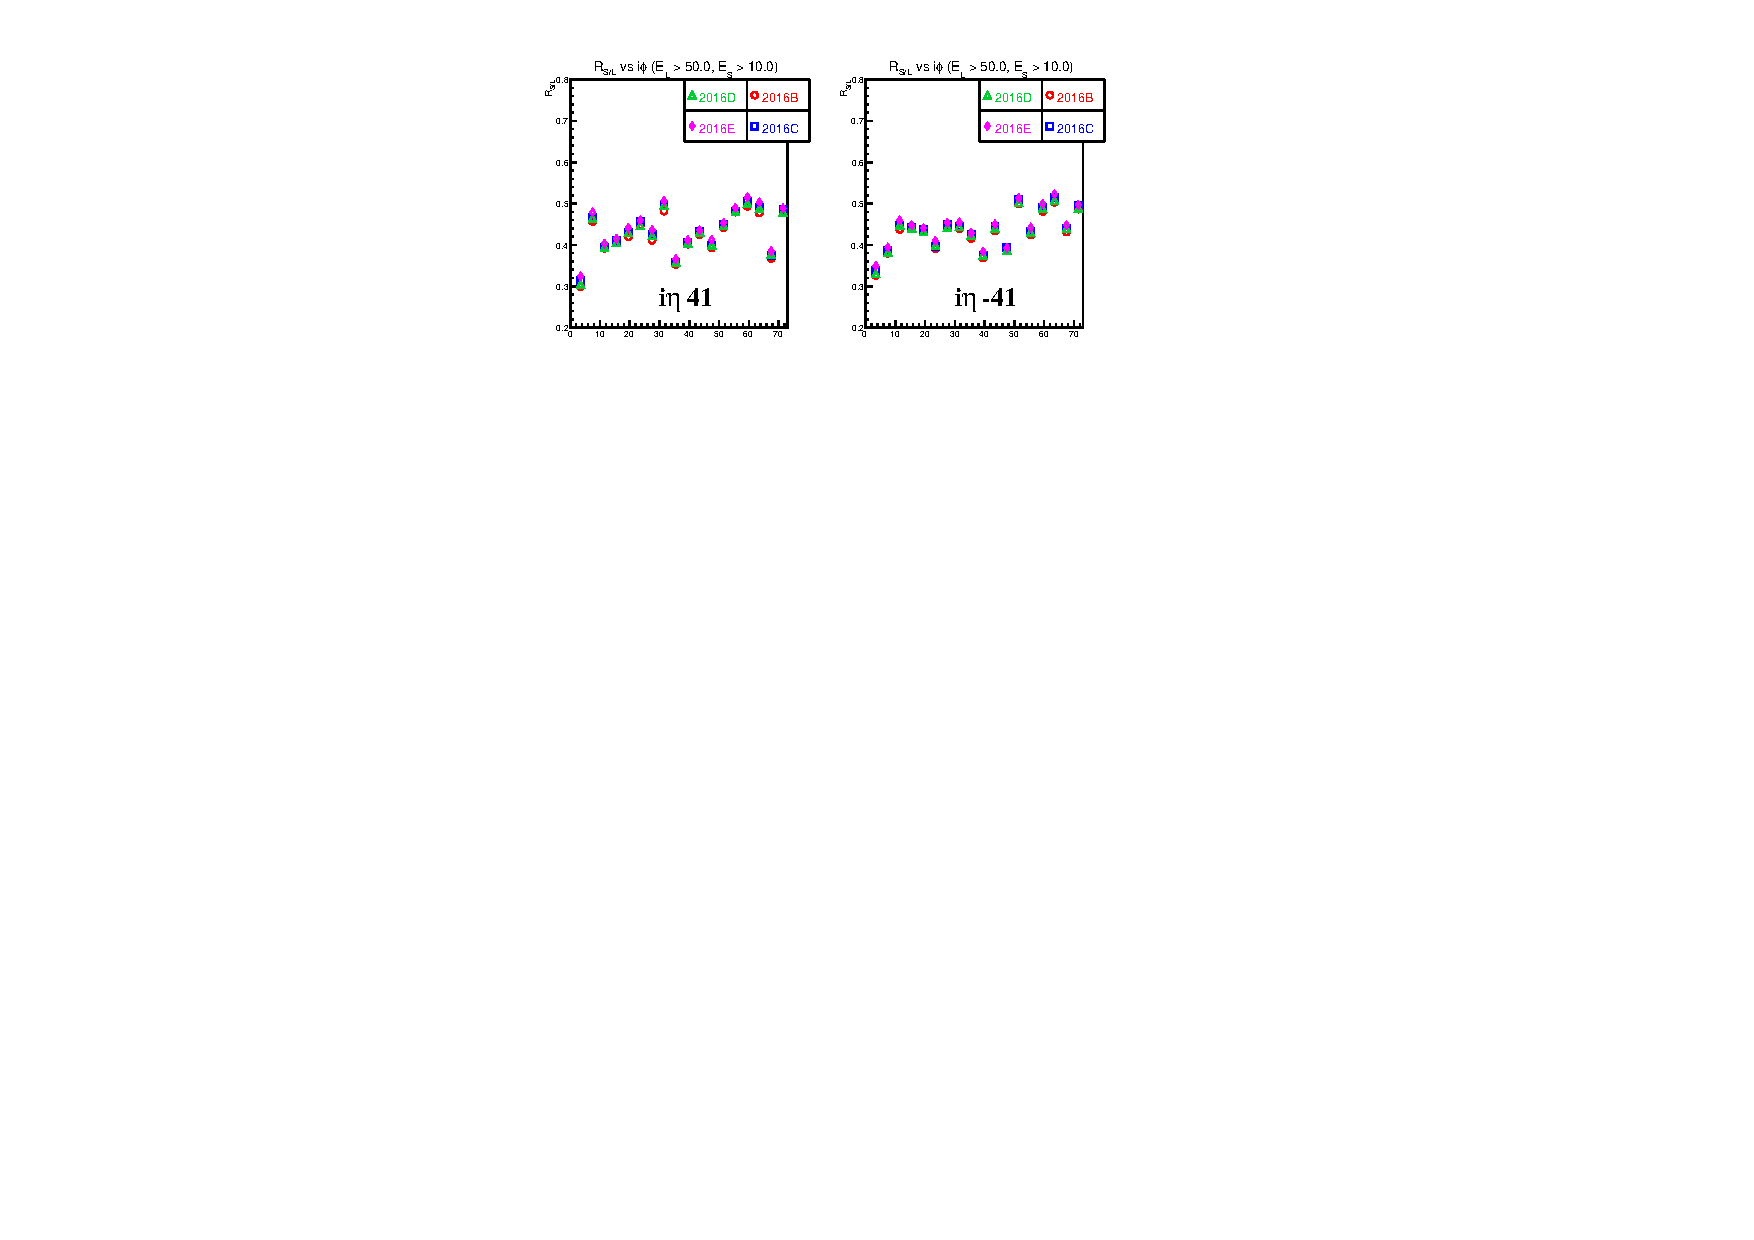
\includegraphics[width=0.99\linewidth]{../Figures/Chap2/ImageFiles_HF/Ratio/2016/Corrected/2016BtoE/ieta41_E1E2Cut3Ietaiphi}
\caption{\ratiosl vs $i\phi$ for $|i\eta|$ 41 for 2016BtoE(Correction NOT applied)}
\label{fig:ieta41_E1E2Cut3IetaiphiBtoE}
\end{figure}
\begin{figure}[h!]
\centering
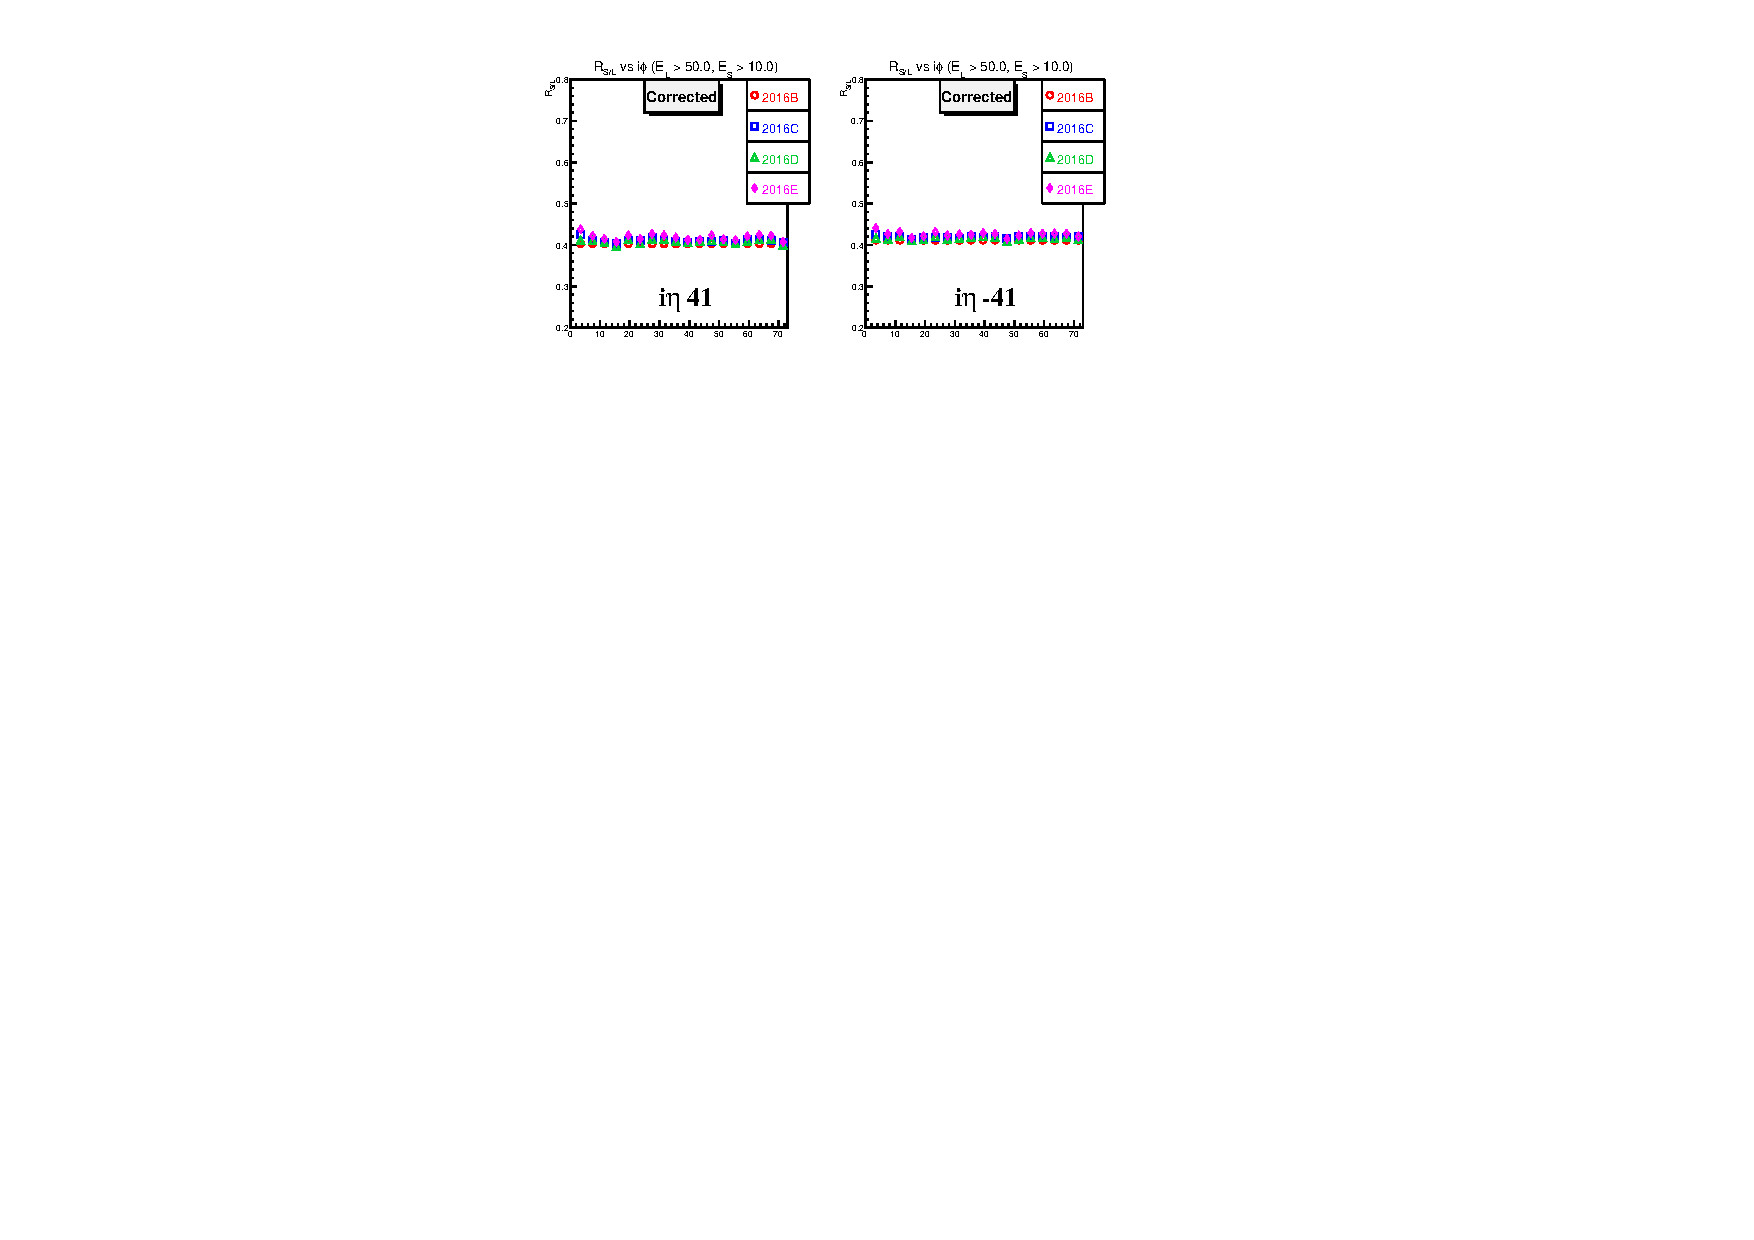
\includegraphics[width=0.99\linewidth]{../Figures/Chap2/ImageFiles_HF/Ratio/2016/Corrected/2016BtoE/ieta41_E1E2Cut3Ietaiphi_Crrtd}
\caption{\ratiosl vs $i\phi$ for $|i\eta|$ 41 for 2016BtoE(Correction applied)}
\label{fig:ieta41_E1E2Cut3Ietaiphi_CrrtdBtoE}
\end{figure}


%			B,F,G,H
\clearpage
\begin{figure}[h!]
\centering
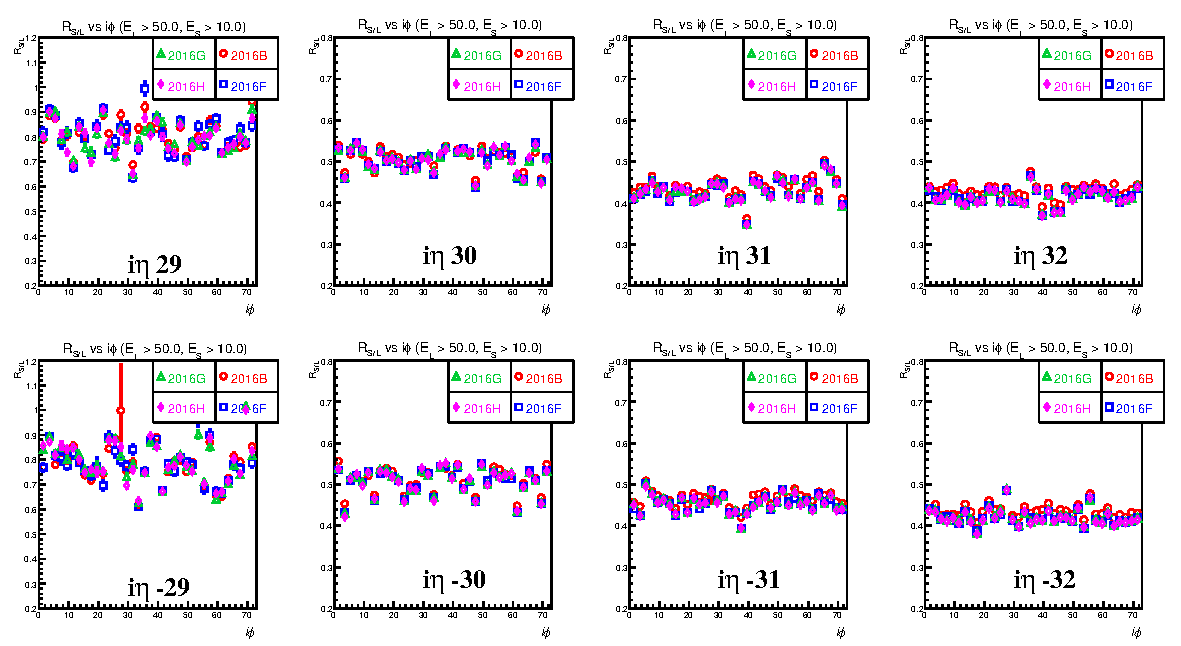
\includegraphics[width=0.99\linewidth]{../Figures/Chap2/ImageFiles_HF/Ratio/2016/Corrected/ieta29_32_E1E2Cut3Ietaiphi}
\caption{\ratiosl vs $i\phi$ for $|i\eta|$ 29 to 32 for 2016B,F,G,H(Correction NOT applied)}
\label{fig:ieta29_32_E1E2Cut3Ietaiphi}
\end{figure}
\begin{figure}[h!]
\centering
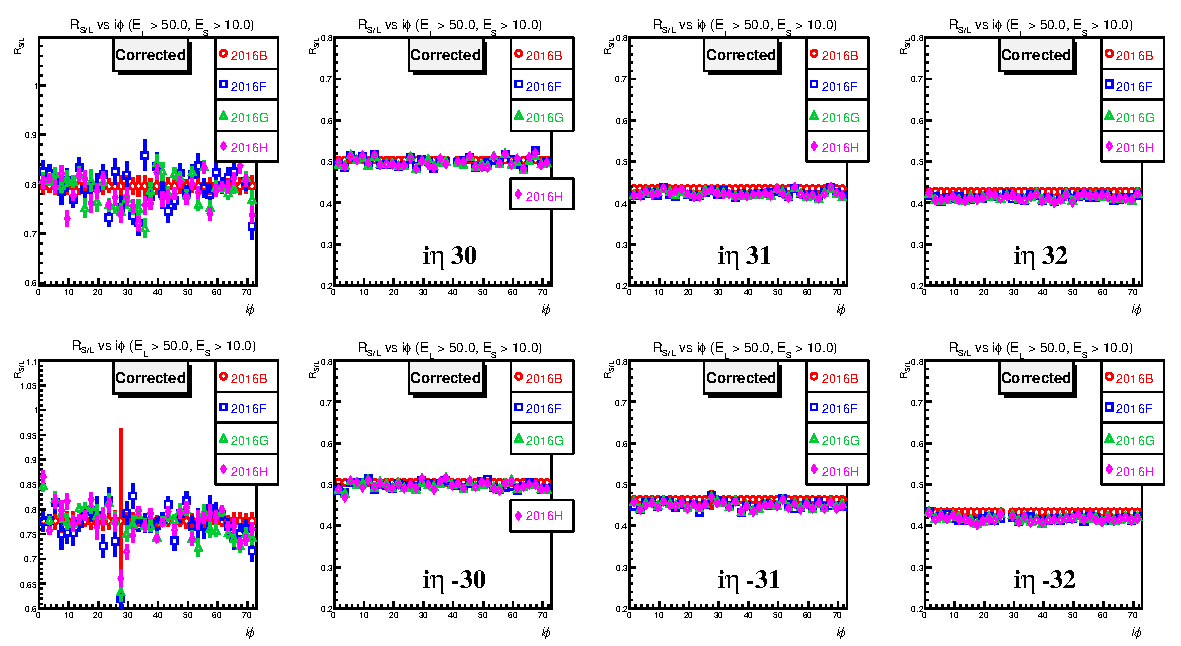
\includegraphics[width=0.99\linewidth]{../Figures/Chap2/ImageFiles_HF/Ratio/2016/Corrected/ieta29_32_E1E2Cut3Ietaiphi_Crrtd}
\caption{\ratiosl vs $i\phi$ for $|i\eta|$ 29 to 32 for 2016B,F,G,H(Correction applied)}
\label{fig:ieta29_32_E1E2Cut3Ietaiphi_Crrtd}
\end{figure}
\newpage
\begin{figure}[h!]
\centering
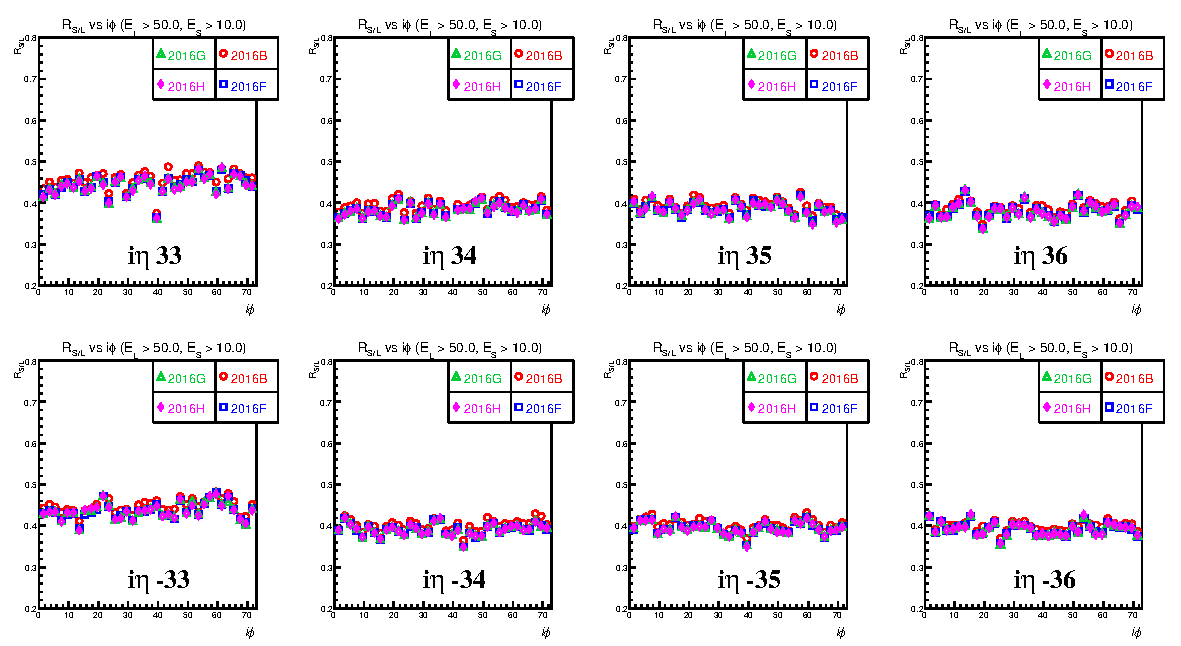
\includegraphics[width=0.99\linewidth]{../Figures/Chap2/ImageFiles_HF/Ratio/2016/Corrected/ieta33_36_E1E2Cut3Ietaiphi}
\caption{\ratiosl vs $i\phi$ for $|i\eta|$ 33 to 36 for 2016B,F,G,H(Correction NOT applied)}
\label{fig:ieta33_36_E1E2Cut3Ietaiphi}
\end{figure}
\begin{figure}[h!]
\centering
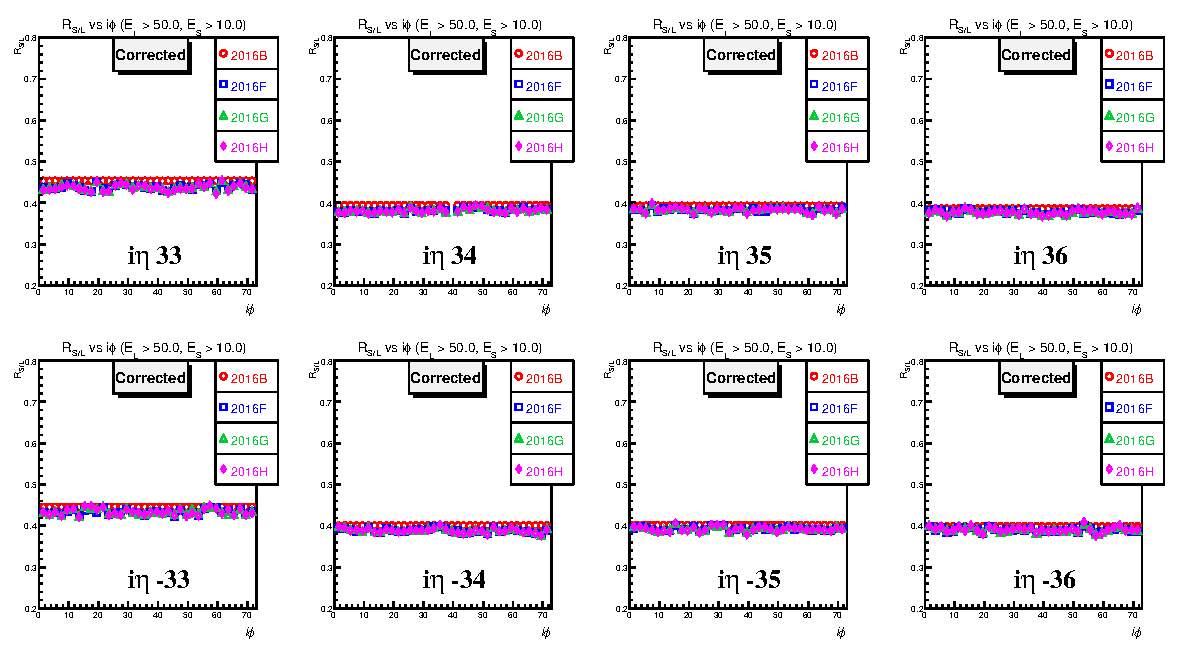
\includegraphics[width=0.99\linewidth]{../Figures/Chap2/ImageFiles_HF/Ratio/2016/Corrected/ieta33_36_E1E2Cut3Ietaiphi_Crrtd}
\caption{\ratiosl vs $i\phi$ for $|i\eta|$ 33 to 36 for 2016B,F,G,H(Correction applied)}
\label{fig:ieta33_36_E1E2Cut3Ietaiphi_Crrtd}
\end{figure}
\newpage
\begin{figure}[h!]
\centering
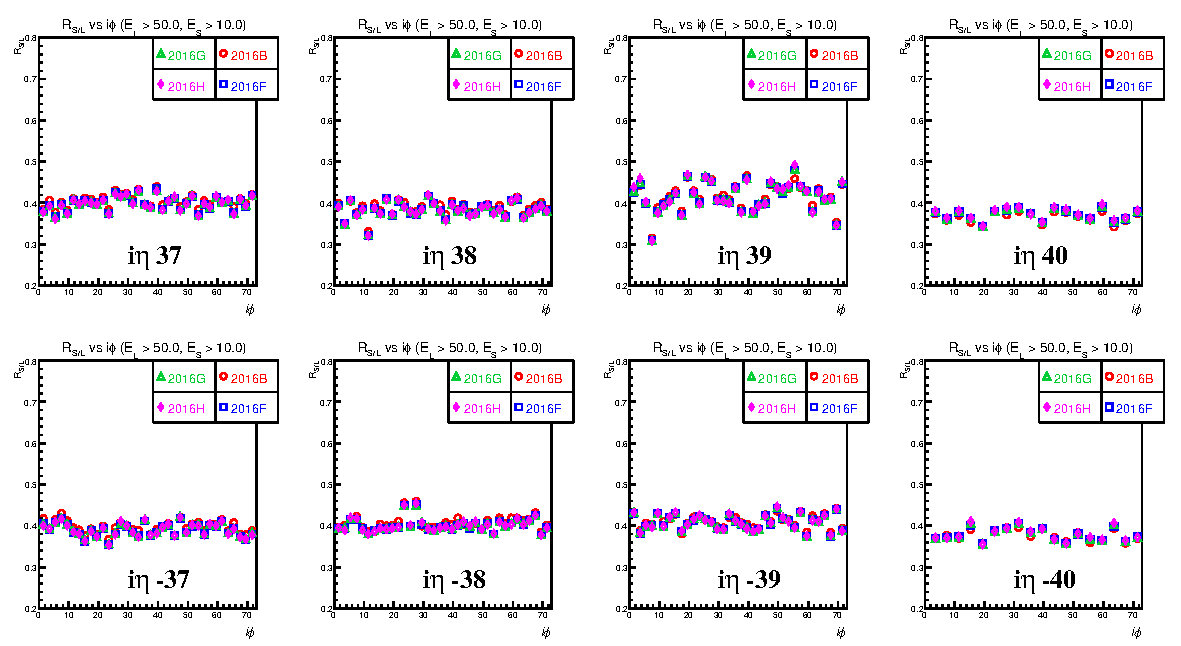
\includegraphics[width=0.99\linewidth]{../Figures/Chap2/ImageFiles_HF/Ratio/2016/Corrected/ieta37_40_E1E2Cut3Ietaiphi}
\caption{\ratiosl vs $i\phi$ for $|i\eta|$ 37 to 40 for 2016B,F,G,H(Correction NOT applied)}
\label{fig:ieta37_40_E1E2Cut3Ietaiphi}
\end{figure}
\begin{figure}[h!]
\centering
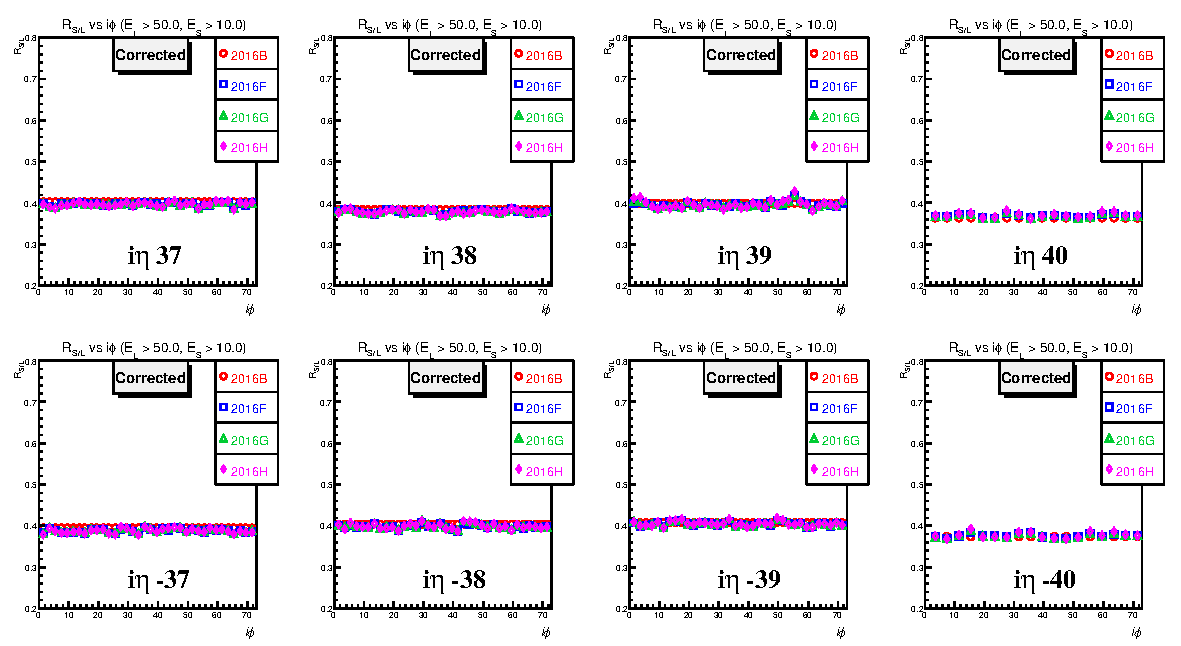
\includegraphics[width=0.99\linewidth]{../Figures/Chap2/ImageFiles_HF/Ratio/2016/Corrected/ieta37_40_E1E2Cut3Ietaiphi_Crrtd}
\caption{\ratiosl vs $i\phi$ for $|i\eta|$ 33 to 36 for 2016B,F,G,H(Correction applied)}
\label{fig:ieta37_40_E1E2Cut3Ietaiphi_Crrtd}
\end{figure}
\newpage
\begin{figure}[h!]
\centering
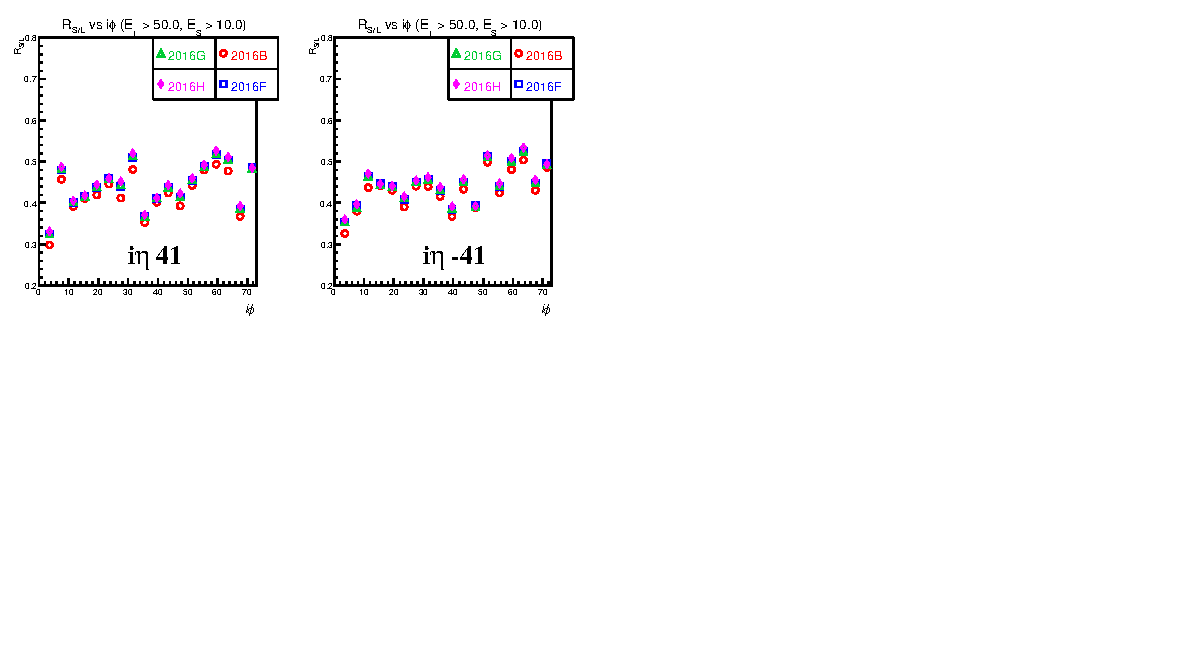
\includegraphics[width=0.99\linewidth]{../Figures/Chap2/ImageFiles_HF/Ratio/2016/Corrected/ieta41_E1E2Cut3Ietaiphi}
\caption{\ratiosl vs $i\phi$ for $|i\eta|$ 41 for 2016B,F,G,H(Correction NOT applied)}
\label{fig:ieta41_E1E2Cut3Ietaiphi}
\end{figure}
\begin{figure}[h!]
\centering
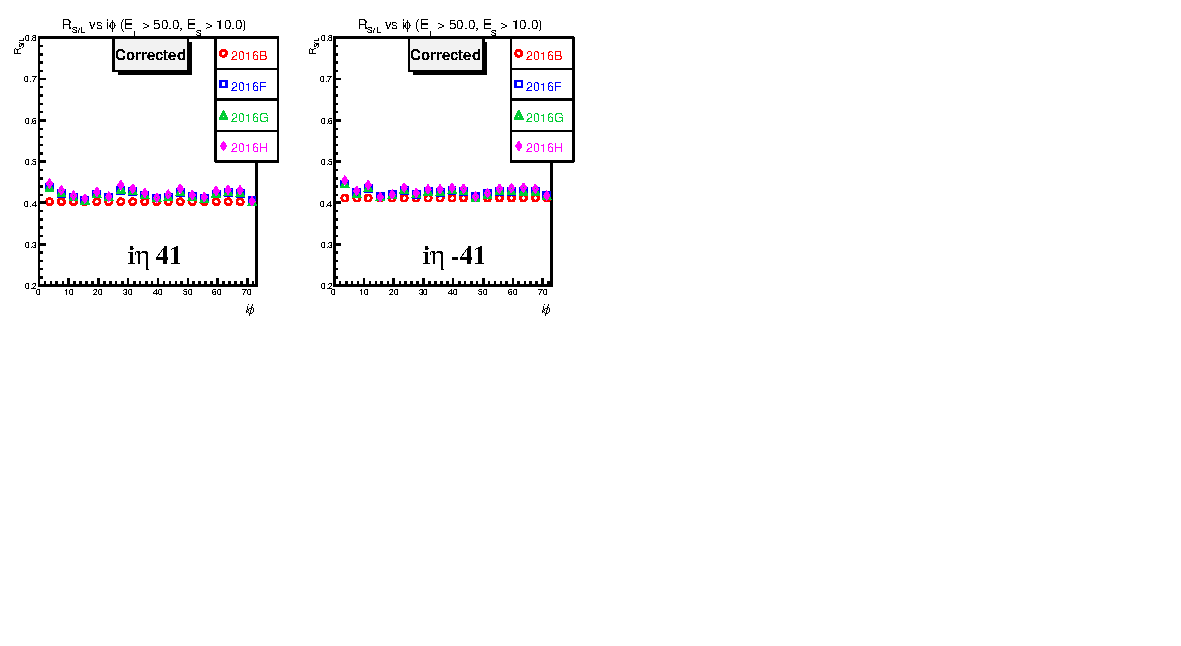
\includegraphics[width=0.99\linewidth]{../Figures/Chap2/ImageFiles_HF/Ratio/2016/Corrected/ieta41_E1E2Cut3Ietaiphi_Crrtd}
\caption{\ratiosl vs $i\phi$ for $|i\eta|$ 41 for 2016B,F,G,H(Correction applied)}
\label{fig:ieta41_E1E2Cut3Ietaiphi_Crrtd}
\end{figure}

% Correction on 2016B with different energy thresholds
\clearpage
\begin{figure}[h!]
\centering
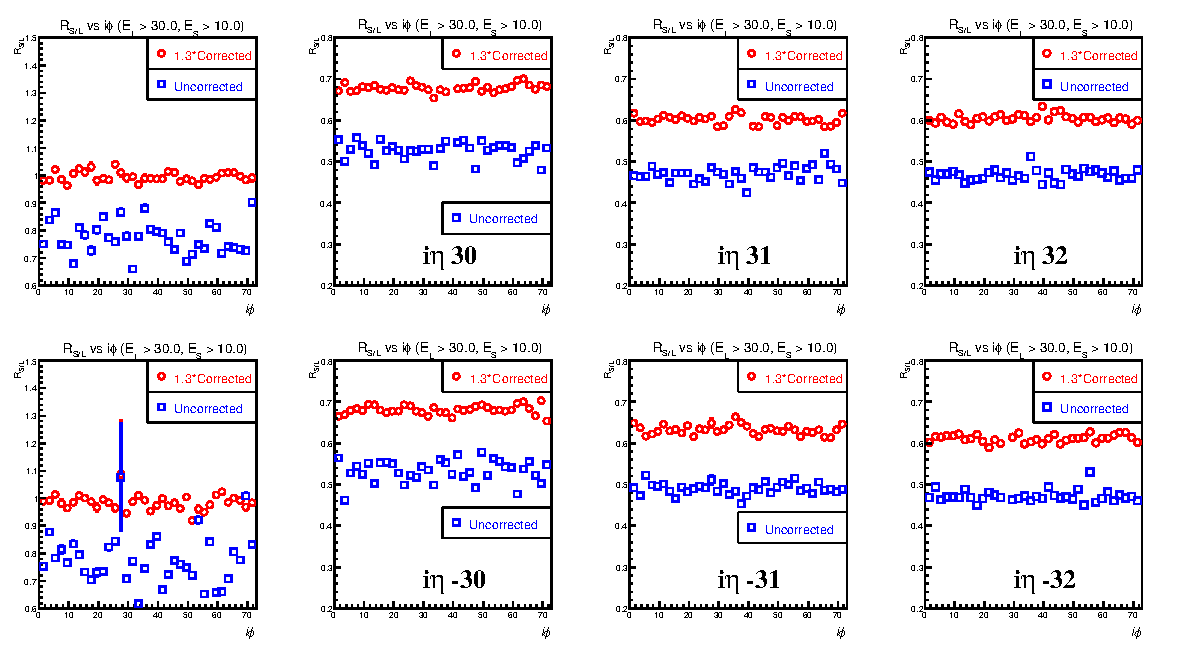
\includegraphics[width=0.99\linewidth]{../Figures/Chap2/ImageFiles_HF/Ratio/2016/Corrected/EnegyCut3010/ieta29_32_E1E2Cut1Ietaiphi_Crrtd}
\caption{\ratiosl vs $i\phi$ for $|i\eta|$ 29 to 32 for 2016B(Corrections obtained using $(E_{long},E_{short})>(50,10)$ and applied on $(E_{long},E_{short})>(30,10)$)}
\label{fig:ieta29_32_E1E2Cut1Ietaiphi_Crrtd}
\end{figure}
\begin{figure}[h!]
\centering
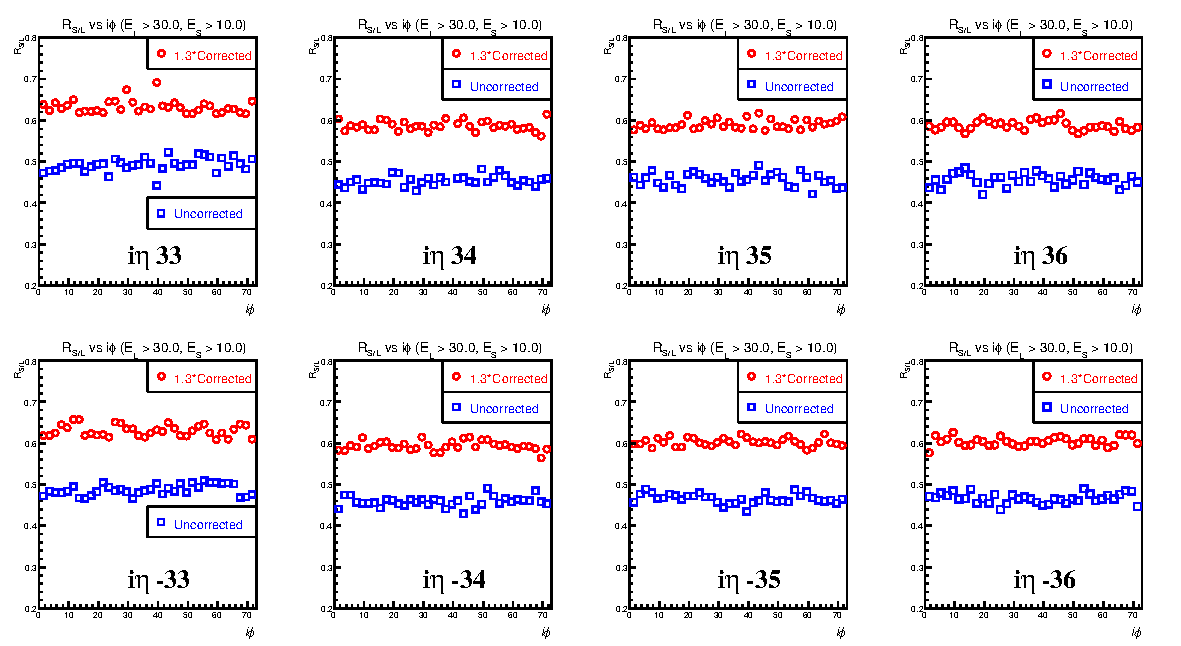
\includegraphics[width=0.99\linewidth]{../Figures/Chap2/ImageFiles_HF/Ratio/2016/Corrected/EnegyCut3010/ieta33_36_E1E2Cut1Ietaiphi_Crrtd}
\caption{\ratiosl vs $i\phi$ for $|i\eta|$ 33 to 36 for 2016B(Corrections obtained using $(E_{long},E_{short})>(50,10)$ and applied on $(E_{long},E_{short})>(30,10)$)}
\label{fig:ieta33_36_E1E2Cut1Ietaiphi_Crrtd}
\end{figure}
\begin{figure}[h!]
\centering
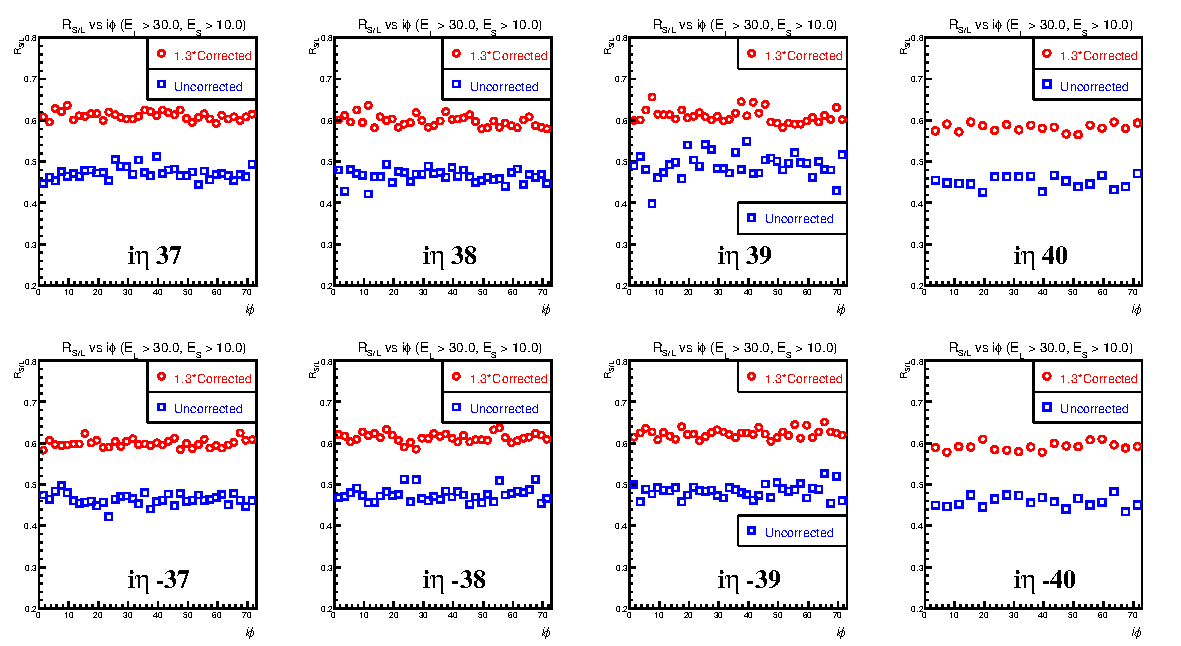
\includegraphics[width=0.99\linewidth]{../Figures/Chap2/ImageFiles_HF/Ratio/2016/Corrected/EnegyCut3010/ieta37_40_E1E2Cut1Ietaiphi_Crrtd}
\caption{\ratiosl vs $i\phi$ for $|i\eta|$ 37 to 40 for 2016B(Corrections obtained using $(E_{long},E_{short})>(50,10)$ and applied on $(E_{long},E_{short})>(30,10)$)}
\label{fig:ieta37_40_E1E2Cut1Ietaiphi_Crrtd}
\end{figure}
\begin{figure}[h!]
\centering
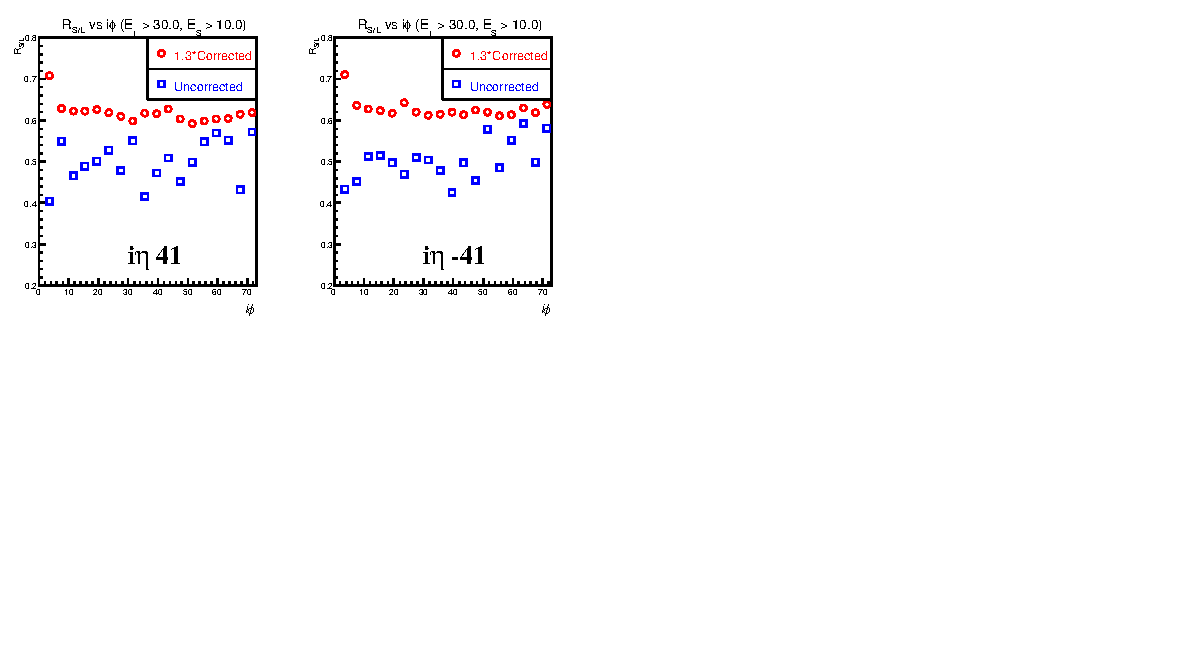
\includegraphics[width=0.99\linewidth]{../Figures/Chap2/ImageFiles_HF/Ratio/2016/Corrected/EnegyCut3010/ieta41_E1E2Cut1Ietaiphi_Crrtd}
\caption{\ratiosl vs $i\phi$ for $|i\eta|$ 41 for 2016B(Corrections obtained using $(E_{long},E_{short})>(50,10)$ and applied on $(E_{long},E_{short})>(30,10)$)}
\label{fig:ieta41_E1E2Cut1Ietaiphi_Crrtd}
\end{figure}
\clearpage
\begin{figure}[h!]
\centering
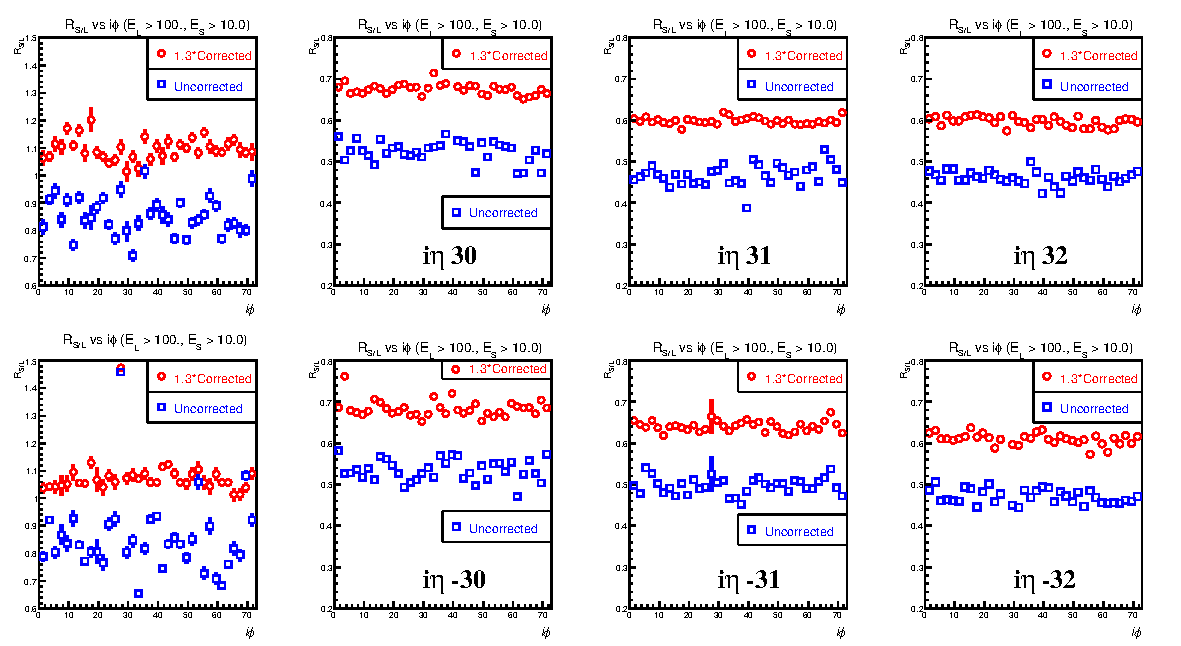
\includegraphics[width=0.99\linewidth]{../Figures/Chap2/ImageFiles_HF/Ratio/2016/Corrected/EnergyCut10010/ieta29_32_E1E2Cut4Ietaiphi_Crrtd}
\caption{\ratiosl vs $i\phi$ for $|i\eta|$ 29 to 32 for 2016B(Corrections obtained using $(E_{long},E_{short})>(50,10)$ and applied on $(E_{long},E_{short})>(100,10)$)}
\label{fig:ieta29_32_E1E2Cut4Ietaiphi_Crrtd}
\end{figure}
\begin{figure}[h!]
\centering
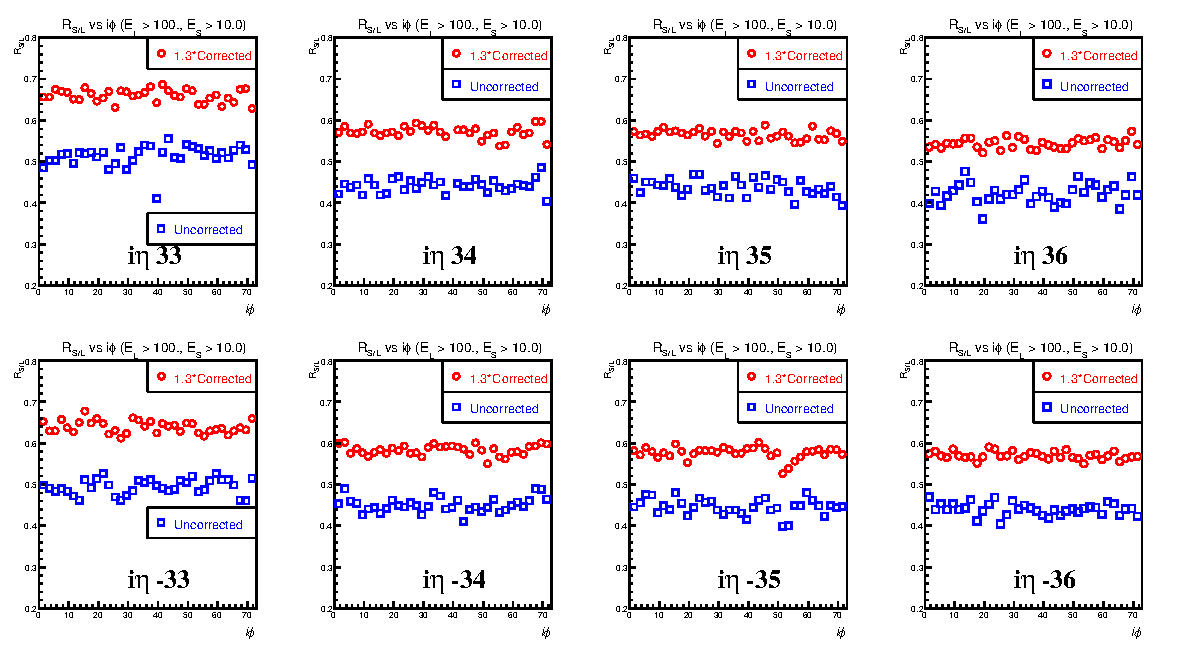
\includegraphics[width=0.99\linewidth]{../Figures/Chap2/ImageFiles_HF/Ratio/2016/Corrected/EnergyCut10010/ieta33_36_E1E2Cut4Ietaiphi_Crrtd}
\caption{\ratiosl vs $i\phi$ for $|i\eta|$ 33 to 36 for 2016B(Corrections obtained using $(E_{long},E_{short})>(50,10)$ and applied on $(E_{long},E_{short})>(100,10)$)}
\label{fig:ieta33_36_E1E2Cut4Ietaiphi_Crrtd}
\end{figure}
\begin{figure}[h!]
\centering
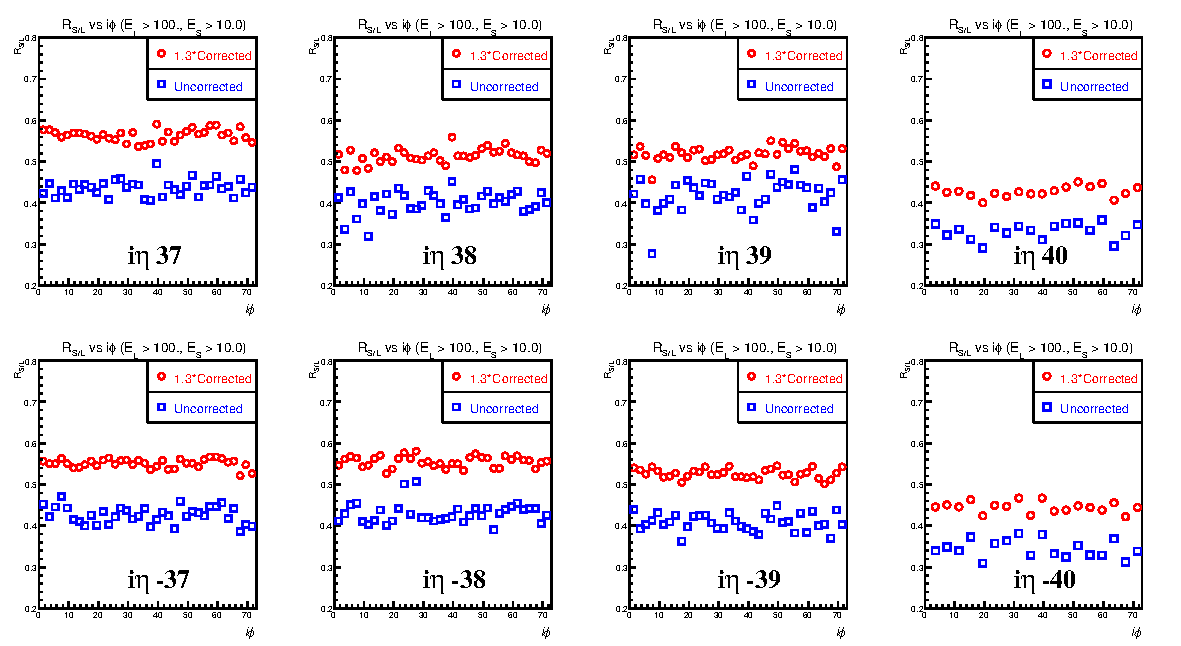
\includegraphics[width=0.99\linewidth]{../Figures/Chap2/ImageFiles_HF/Ratio/2016/Corrected/EnergyCut10010/ieta37_40_E1E2Cut4Ietaiphi_Crrtd}
\caption{\ratiosl vs $i\phi$ for $|i\eta|$ 37 to 40 for 2016B(Corrections obtained using $(E_{long},E_{short})>(50,10)$ and applied on $(E_{long},E_{short})>(100,10)$)}
\label{fig:ieta37_40_E1E2Cut4Ietaiphi_Crrtd}
\end{figure}
\begin{figure}[h!]
\centering
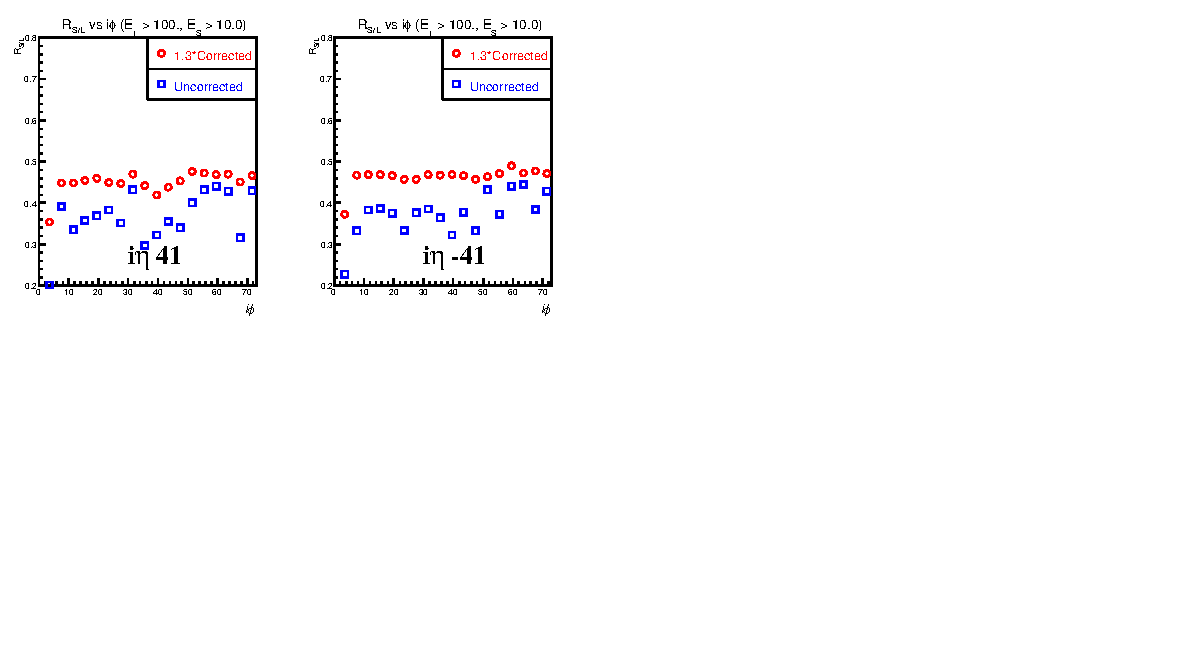
\includegraphics[width=0.99\linewidth]{../Figures/Chap2/ImageFiles_HF/Ratio/2016/Corrected/EnergyCut10010/ieta41_E1E2Cut4Ietaiphi_Crrtd}
\caption{\ratiosl vs $i\phi$ for $|i\eta|$ 41 for 2016B(Corrections obtained using $(E_{long},E_{short})>(50,10)$ and applied on $(E_{long},E_{short})>(100,10)$)}
\label{fig:ieta41_E1E2Cut4Ietaiphi_Crrtd}
\end{figure}

\newpage
\begin{table}[!hp] 
\centering
\caption{Inter-calibration correction factors for $+i\eta$}
\label{tab:corrFacPosEta}
\begin{tabular}{c|ccccccccccccc}
\hline \hline
$i\phi,i\eta$ & 29 & 30 & 31 & 32 & 33 & 34 & 35 & 36 & 37 & 38 & 39 & 40 & 41 \\
\hline
1 & 1.006 & 0.934 & 1.020 & 0.971 & 1.041 & 1.043 & 0.960 & 1.032 & 1.049 & 0.964 & 0.941 \\
3 & 0.900 & 1.062 & 0.990 & 1.001 & 1.005 & 1.011 & 1.021 & 0.972 & 0.992 & 1.100 & 0.902 & 0.973 & 1.349 \\
5 & 0.909 & 0.972 & 0.990 & 0.993 & 1.033 & 1.001 & 0.966 & 1.039 & 1.067 & 0.951 & 0.998 \\
7 & 1.011 & 0.926 & 0.935 & 0.977 & 0.997 & 0.983 & 0.955 & 1.003 & 1.003 & 1.020 & 1.267 & 1.014 & 0.882 \\
9 & 0.989 & 0.972 & 0.989 & 0.955 & 0.990 & 1.048 & 0.995 & 0.972 & 1.052 & 0.979 & 1.025 \\
11 & 1.140 & 1.005 & 0.995 & 1.013 & 1.009 & 0.989 & 1.013 & 0.944 & 0.981 & 1.162 & 0.996 & 0.982 & 1.029 \\
13 & 0.974 & 1.067 & 1.038 & 1.025 & 0.959 & 0.987 & 0.958 & 0.901 & 1.013 & 0.965 & 0.959 \\
15 & 0.995 & 0.938 & 0.980 & 0.996 & 1.006 & 1.035 & 1.008 & 0.953 & 0.980 & 1.009 & 0.930 & 1.029 & 0.980 \\
17 & 1.092 & 0.983 & 0.996 & 1.018 & 0.980 & 1.035 & 1.046 & 1.020 & 0.986 & 0.934 & 1.048 \\
19 & 0.942 & 0.973 & 0.985 & 1.018 & 0.972 & 0.959 & 1.001 & 1.108 & 1.003 & 1.032 & 0.862 & 1.060 & 0.960 \\
21 & 0.896 & 0.984 & 1.032 & 0.972 & 0.962 & 0.936 & 0.937 & 1.026 & 0.973 & 0.942 & 0.929 \\
23 & 0.979 & 1.023 & 1.019 & 0.976 & 1.071 & 1.044 & 0.952 & 0.983 & 1.051 & 0.959 & 0.975 & 0.956 & 0.903 \\
25 & 1.054 & 1.015 & 1.027 & 1.022 & 0.981 & 0.973 & 1.004 & 0.989 & 0.935 & 1.011 & 0.863 \\
27 & 0.896 & 1.002 & 0.966 & 0.976 & 0.967 & 1.048 & 1.011 & 1.030 & 0.955 & 1.013 & 0.873 & 0.978 & 0.980 \\
29 & 0.978 & 0.988 & 0.948 & 1.020 & 1.070 & 1.002 & 1.009 & 0.979 & 0.952 & 0.983 & 0.970 \\
31 & 1.159 & 0.978 & 0.962 & 1.012 & 1.007 & 0.956 & 0.996 & 0.997 & 0.987 & 0.919 & 0.951 & 0.957 & 0.837 \\
33 & 0.955 & 1.027 & 1.053 & 1.023 & 0.970 & 1.021 & 1.045 & 0.935 & 0.931 & 0.959 & 0.979 \\
35 & 0.864 & 0.976 & 1.012 & 0.897 & 0.951 & 0.974 & 0.951 & 1.023 & 1.015 & 0.972 & 0.908 & 0.973 & 1.143 \\
37 & 0.946 & 0.937 & 1.033 & 0.975 & 0.974 & 1.030 & 0.989 & 0.976 & 1.026 & 1.033 & 1.030 \\
39 & 0.953 & - & 1.199 & 1.095 & 1.205 & - & 1.027 & 0.981 & 0.918 & 0.953 & 0.856 & 1.045 & 1.003 \\
41 & 0.961 & 0.952 & 0.929 & 0.980 & 1.009 & 0.991 & 0.953 & 1.007 & 1.020 & 0.999 & 1.050 \\
43 & 1.028 & 0.944 & 0.947 & 1.065 & 0.930 & 1.010 & 0.967 & 1.054 & 0.993 & 0.970 & 1.005 & 0.960 & 0.948 \\
45 & 1.065 & 0.980 & 0.988 & 1.080 & 0.996 & 0.997 & 0.973 & 1.019 & 0.978 & 1.018 & 0.976 \\
47 & 0.950 & 1.107 & 1.010 & 0.973 & 0.994 & 0.976 & 0.990 & 1.025 & 1.030 & 1.021 & 0.900 & 0.962 & 1.026 \\
49 & 1.104 & 0.936 & 0.930 & 0.988 & 0.962 & 0.951 & 0.947 & 0.971 & 0.999 & 0.982 & 0.908 \\
51 & 1.056 & 0.991 & 0.940 & 0.987 & 0.962 & 1.020 & 0.974 & 0.918 & 0.962 & 0.969 & 0.932 & 0.988 & 0.912 \\
53 & 0.993 & 0.959 & 0.989 & 0.967 & 0.925 & 0.968 & 1.013 & 0.994 & 1.050 & 1.009 & 0.919 \\
55 & 1.037 & 0.962 & 0.958 & 0.979 & 0.954 & 0.946 & 1.058 & 0.950 & 0.993 & 0.977 & 0.870 & 1.014 & 0.840 \\
57 & 0.918 & 0.967 & 1.028 & 0.959 & 0.955 & 0.967 & 0.923 & 0.969 & 1.018 & 1.036 & 0.913 \\
59 & 0.942 & 0.982 & 0.950 & 0.980 & 1.003 & 1.011 & 0.999 & 0.986 & 0.973 & 0.954 & 0.927 & 0.956 & 0.817 \\
61 & 1.082 & 1.077 & 0.933 & 1.010 & 0.936 & 1.006 & 1.064 & 0.986 & 1.000 & 0.928 & 1.011 \\
63 & 1.047 & 1.062 & 1.014 & 0.959 & 0.989 & 0.984 & 0.985 & 0.957 & 0.996 & 1.040 & 0.918 & 1.061 & 0.844 \\
65 & 1.051 & 1.004 & 0.863 & 1.021 & 0.938 & 0.996 & 1.007 & 1.065 & 1.028 & 0.999 & 0.978 \\
67 & 1.048 & 0.963 & 0.913 & 1.008 & 0.962 & 0.994 & 1.005 & 1.009 & 0.982 & 0.977 & 0.964 & 1.016 & 1.096 \\
69 & 1.040 & 1.098 & 0.950 & 0.989 & 0.984 & 0.946 & 1.057 & 0.952 & 1.010 & 0.957 & 1.131 \\
71 & 0.845 & 0.984 & 1.060 & 0.962 & 0.982 & 1.029 & 1.071 & 0.995 & 0.959 & 0.997 & 0.897 & 0.969 & 0.833 \\

\hline \hline
\end{tabular}
\end{table}

\begin{table}[!hp]
\centering
\caption{Inter-calibration correction factors for $-i\eta$}
\label{tab:corrFacNegEta}
\begin{tabular}{c|ccccccccccccc}
\hline \hline
$i\phi,i\eta$ & -29 & -30 & -31 & -32 & -33 & -34 & -35 & -36 & -37 & -38 & -39 & -40 & -41 \\
\hline 
1 & 1.009 & 0.907 & 1.013 & 0.988 & 1.006 & 1.017 & 1.006 & 0.941 & 0.946 & 1.020 & 0.946 \\
3 & 0.869 & 1.112 & 1.035 & 0.958 & 0.986 & 0.943 & 0.965 & 1.016 & 1.004 & 1.007 & 1.049 & 1.010 & 1.262 \\
5 & 0.996 & 0.989 & 0.909 & 1.020 & 1.000 & 0.964 & 0.954 & 0.966 & 0.950 & 0.968 & 1.002 \\
7 & 0.928 & 0.966 & 0.958 & 1.014 & 1.033 & 0.995 & 0.939 & 0.991 & 0.919 & 0.956 & 1.009 & 0.994 & 1.083 \\
9 & 0.969 & 0.993 & 0.976 & 1.013 & 1.014 & 1.038 & 1.009 & 0.993 & 0.955 & 1.018 & 0.950 \\
11 & 0.909 & 0.968 & 0.991 & 1.022 & 1.021 & 0.993 & 0.990 & 0.996 & 1.000 & 1.045 & 0.990 & 1.009 & 0.940 \\
13 & 0.977 & 1.062 & 1.003 & 0.959 & 1.084 & 1.001 & 0.997 & 0.980 & 1.014 & 1.049 & 0.978 \\
15 & 1.051 & 0.946 & 1.046 & 1.001 & 1.020 & 1.044 & 0.960 & 0.939 & 1.050 & 1.001 & 0.954 & 0.956 & 0.931 \\
17 & 1.079 & 0.936 & 0.974 & 1.061 & 1.013 & 1.002 & 0.982 & 1.030 & 1.005 & 1.008 & 1.073 \\
19 & 1.018 & 0.947 & 1.024 & 0.997 & 0.987 & 0.981 & 1.000 & 1.000 & 1.043 & 1.007 & 1.005 & 1.051 & 0.954 \\
21 & 1.043 & 0.987 & 0.968 & 0.942 & 0.946 & 0.996 & 0.995 & 1.005 & 0.991 & 0.980 & 0.968 \\
23 & 0.919 & 1.069 & 0.983 & 0.987 & 0.958 & 1.024 & 0.962 & 0.963 & 1.076 & 0.887 & 0.961 & 0.968 & 1.053 \\
25 & 0.880 & 1.015 & 0.989 & 0.984 & 1.034 & 0.971 & 0.980 & 1.080 & 1.001 & 1.010 & 0.981 \\
27 & 0.777 & 1.008 & 0.974 & - & 1.020 & 0.987 & 0.973 & 1.026 & 0.967 & 0.880 & 0.991 & 0.946 & 0.933 \\
29 & 1.026 & 0.953 & 0.998 & 1.020 & 1.013 & 1.021 & 1.014 & 0.971 & 0.985 & 1.010 & 1.025 \\
31 & 0.984 & 0.955 & 0.968 & 1.030 & 1.049 & 1.015 & 1.059 & 0.979 & 1.009 & 1.019 & 1.034 & 0.943 & 0.937 \\
33 & 1.257 & 1.059 & 1.040 & 0.973 & 0.991 & 0.958 & 1.026 & 0.972 & 1.015 & 1.018 & 0.970 \\
35 & 1.025 & 0.927 & 1.057 & 1.007 & 0.977 & 0.962 & 1.008 & 1.000 & 0.959 & 1.021 & 0.969 & 0.996 & 0.989 \\
37 & 0.881 & 0.937 & 1.102 & 0.995 & 0.983 & 1.031 & 1.029 & 1.017 & 1.038 & 0.989 & 1.000 \\
39 & 0.871 & 0.968 & 1.044 & 0.986 & 0.968 & 1.026 & 1.086 & 1.026 & 1.009 & 1.003 & 1.009 & 0.949 & 1.117 \\
41 & 1.151 & 0.919 & 0.974 & 0.952 & 1.014 & 0.983 & 1.018 & 1.030 & 0.991 & 0.962 & 1.034 \\
43 & 1.035 & 1.004 & 0.970 & 1.009 & 1.018 & 1.096 & 1.002 & 1.017 & 0.974 & 1.002 & 1.037 & 1.007 & 0.949 \\
45 & 0.978 & 0.991 & 0.961 & 0.985 & 1.014 & 1.003 & 0.966 & 1.023 & 1.051 & 1.025 & 0.955 \\
47 & 0.975 & 1.077 & 1.020 & 0.995 & 0.947 & 1.035 & 0.999 & 1.032 & 0.939 & 0.997 & 0.994 & 1.035 & 1.056 \\
49 & 1.033 & 0.921 & 0.980 & 1.015 & 0.987 & 1.033 & 1.000 & 0.986 & 1.003 & 1.027 & 0.936 \\
51 & 0.981 & 1.009 & 0.956 & 0.963 & 0.959 & 0.952 & 1.015 & 1.002 & 0.978 & 0.979 & 0.985 & 0.978 & 0.824 \\
53 & 0.802 & 0.929 & 0.986 & 1.046 & 0.998 & 0.975 & 1.037 & 0.957 & 0.967 & 1.061 & 0.982 \\
55 & 1.119 & 0.940 & 0.945 & 0.909 & 0.974 & 1.006 & 0.954 & 0.986 & 1.015 & 0.963 & 1.019 & 1.038 & 0.970 \\
57 & 0.893 & 0.960 & 0.978 & 1.013 & 0.952 & 0.985 & 0.972 & 0.992 & 0.976 & 0.995 & 0.938 \\
59 & 1.181 & 0.966 & 0.986 & 1.009 & 0.926 & 0.990 & 0.930 & 1.006 & 0.976 & 0.964 & 1.059 & 1.027 & 0.855 \\
61 & 1.191 & 1.125 & 1.006 & 0.977 & 0.957 & 0.974 & 0.968 & 0.957 & 0.952 & 0.964 & 0.961 \\
63 & 1.071 & 1.003 & 0.961 & 1.033 & 0.931 & 0.987 & 1.002 & 0.984 & 1.017 & 0.979 & 0.988 & 0.950 & 0.817 \\
65 & 0.954 & 0.946 & 0.974 & 1.014 & 0.972 & 0.986 & 1.042 & 1.004 & 0.967 & 0.969 & 0.952 \\
67 & 0.983 & 0.981 & 0.965 & 1.030 & 1.060 & 0.932 & 1.000 & 0.982 & 1.039 & 0.936 & 1.063 & 1.040 & 0.954 \\
69 & 0.738 & 1.076 & 1.009 & 1.002 & 1.054 & 0.946 & 1.013 & 0.987 & 1.044 & 1.048 & 0.925 \\
71 & 0.910 & 0.919 & 1.018 & 1.006 & 0.986 & 0.992 & 0.985 & 1.032 & 1.014 & 1.006 & 1.035 & 1.010 & 0.845 \\
\hline \hline
\end{tabular}
\end{table}